\documentclass[]{book}
\usepackage{lmodern}
\usepackage{amssymb,amsmath}
\usepackage{ifxetex,ifluatex}
\usepackage{fixltx2e} % provides \textsubscript
\ifnum 0\ifxetex 1\fi\ifluatex 1\fi=0 % if pdftex
  \usepackage[T1]{fontenc}
  \usepackage[utf8]{inputenc}
\else % if luatex or xelatex
  \ifxetex
    \usepackage{mathspec}
  \else
    \usepackage{fontspec}
  \fi
  \defaultfontfeatures{Ligatures=TeX,Scale=MatchLowercase}
  \newcommand{\euro}{€}
\fi
% use upquote if available, for straight quotes in verbatim environments
\IfFileExists{upquote.sty}{\usepackage{upquote}}{}
% use microtype if available
\IfFileExists{microtype.sty}{%
\usepackage{microtype}
\UseMicrotypeSet[protrusion]{basicmath} % disable protrusion for tt fonts
}{}
\usepackage[margin=1in]{geometry}
\usepackage{hyperref}
\PassOptionsToPackage{usenames,dvipsnames}{color} % color is loaded by hyperref
\hypersetup{unicode=true,
            pdftitle={Introdução à Análise Multivariada usando R},
            pdfauthor={Marcio Nicolau},
            pdfborder={0 0 0},
            breaklinks=true}
\urlstyle{same}  % don't use monospace font for urls
\usepackage{natbib}
\bibliographystyle{apalike}
\usepackage{color}
\usepackage{fancyvrb}
\newcommand{\VerbBar}{|}
\newcommand{\VERB}{\Verb[commandchars=\\\{\}]}
\DefineVerbatimEnvironment{Highlighting}{Verbatim}{commandchars=\\\{\}}
% Add ',fontsize=\small' for more characters per line
\usepackage{framed}
\definecolor{shadecolor}{RGB}{248,248,248}
\newenvironment{Shaded}{\begin{snugshade}}{\end{snugshade}}
\newcommand{\KeywordTok}[1]{\textcolor[rgb]{0.13,0.29,0.53}{\textbf{{#1}}}}
\newcommand{\DataTypeTok}[1]{\textcolor[rgb]{0.13,0.29,0.53}{{#1}}}
\newcommand{\DecValTok}[1]{\textcolor[rgb]{0.00,0.00,0.81}{{#1}}}
\newcommand{\BaseNTok}[1]{\textcolor[rgb]{0.00,0.00,0.81}{{#1}}}
\newcommand{\FloatTok}[1]{\textcolor[rgb]{0.00,0.00,0.81}{{#1}}}
\newcommand{\ConstantTok}[1]{\textcolor[rgb]{0.00,0.00,0.00}{{#1}}}
\newcommand{\CharTok}[1]{\textcolor[rgb]{0.31,0.60,0.02}{{#1}}}
\newcommand{\SpecialCharTok}[1]{\textcolor[rgb]{0.00,0.00,0.00}{{#1}}}
\newcommand{\StringTok}[1]{\textcolor[rgb]{0.31,0.60,0.02}{{#1}}}
\newcommand{\VerbatimStringTok}[1]{\textcolor[rgb]{0.31,0.60,0.02}{{#1}}}
\newcommand{\SpecialStringTok}[1]{\textcolor[rgb]{0.31,0.60,0.02}{{#1}}}
\newcommand{\ImportTok}[1]{{#1}}
\newcommand{\CommentTok}[1]{\textcolor[rgb]{0.56,0.35,0.01}{\textit{{#1}}}}
\newcommand{\DocumentationTok}[1]{\textcolor[rgb]{0.56,0.35,0.01}{\textbf{\textit{{#1}}}}}
\newcommand{\AnnotationTok}[1]{\textcolor[rgb]{0.56,0.35,0.01}{\textbf{\textit{{#1}}}}}
\newcommand{\CommentVarTok}[1]{\textcolor[rgb]{0.56,0.35,0.01}{\textbf{\textit{{#1}}}}}
\newcommand{\OtherTok}[1]{\textcolor[rgb]{0.56,0.35,0.01}{{#1}}}
\newcommand{\FunctionTok}[1]{\textcolor[rgb]{0.00,0.00,0.00}{{#1}}}
\newcommand{\VariableTok}[1]{\textcolor[rgb]{0.00,0.00,0.00}{{#1}}}
\newcommand{\ControlFlowTok}[1]{\textcolor[rgb]{0.13,0.29,0.53}{\textbf{{#1}}}}
\newcommand{\OperatorTok}[1]{\textcolor[rgb]{0.81,0.36,0.00}{\textbf{{#1}}}}
\newcommand{\BuiltInTok}[1]{{#1}}
\newcommand{\ExtensionTok}[1]{{#1}}
\newcommand{\PreprocessorTok}[1]{\textcolor[rgb]{0.56,0.35,0.01}{\textit{{#1}}}}
\newcommand{\AttributeTok}[1]{\textcolor[rgb]{0.77,0.63,0.00}{{#1}}}
\newcommand{\RegionMarkerTok}[1]{{#1}}
\newcommand{\InformationTok}[1]{\textcolor[rgb]{0.56,0.35,0.01}{\textbf{\textit{{#1}}}}}
\newcommand{\WarningTok}[1]{\textcolor[rgb]{0.56,0.35,0.01}{\textbf{\textit{{#1}}}}}
\newcommand{\AlertTok}[1]{\textcolor[rgb]{0.94,0.16,0.16}{{#1}}}
\newcommand{\ErrorTok}[1]{\textcolor[rgb]{0.64,0.00,0.00}{\textbf{{#1}}}}
\newcommand{\NormalTok}[1]{{#1}}
\usepackage{longtable,booktabs}
\usepackage{graphicx,grffile}
\makeatletter
\def\maxwidth{\ifdim\Gin@nat@width>\linewidth\linewidth\else\Gin@nat@width\fi}
\def\maxheight{\ifdim\Gin@nat@height>\textheight\textheight\else\Gin@nat@height\fi}
\makeatother
% Scale images if necessary, so that they will not overflow the page
% margins by default, and it is still possible to overwrite the defaults
% using explicit options in \includegraphics[width, height, ...]{}
\setkeys{Gin}{width=\maxwidth,height=\maxheight,keepaspectratio}
\setlength{\parindent}{0pt}
\setlength{\parskip}{6pt plus 2pt minus 1pt}
\setlength{\emergencystretch}{3em}  % prevent overfull lines
\providecommand{\tightlist}{%
  \setlength{\itemsep}{0pt}\setlength{\parskip}{0pt}}
\setcounter{secnumdepth}{5}

%%% Use protect on footnotes to avoid problems with footnotes in titles
\let\rmarkdownfootnote\footnote%
\def\footnote{\protect\rmarkdownfootnote}

%%% Change title format to be more compact
\usepackage{titling}

% Create subtitle command for use in maketitle
\newcommand{\subtitle}[1]{
  \posttitle{
    \begin{center}\large#1\end{center}
    }
}

\setlength{\droptitle}{-2em}
  \title{Introdução à Análise Multivariada usando R}
  \pretitle{\vspace{\droptitle}\centering\huge}
  \posttitle{\par}
  \author{Marcio Nicolau}
  \preauthor{\centering\large\emph}
  \postauthor{\par}
  \predate{\centering\large\emph}
  \postdate{\par}
  \date{2016-10-26}


% Redefines (sub)paragraphs to behave more like sections
\ifx\paragraph\undefined\else
\let\oldparagraph\paragraph
\renewcommand{\paragraph}[1]{\oldparagraph{#1}\mbox{}}
\fi
\ifx\subparagraph\undefined\else
\let\oldsubparagraph\subparagraph
\renewcommand{\subparagraph}[1]{\oldsubparagraph{#1}\mbox{}}
\fi

\usepackage{booktabs}

\begin{document}
\maketitle

{
\setcounter{tocdepth}{1}
\tableofcontents
}
\chapter{Pré-requisitos}\label{pre-requisitos}

Antes de iniciar o curso, faz-se nescessário instalar as ferramentas e
pacotes para uso.

Será utilizado o sofware \emph{R version 3.3.1 (2016-06-21)} disponível
em \href{https://cran.r-project.org}{CRAN} e o \emph{RStudio v1.0.44
Preview} disponível em
\href{https://www.rstudio.com/products/rstudio/download/preview/}{RStudio}.

A carga horária total será de 20 horas (3 dias) nos quais os seguintes
tópicos de Análise Multivariada serão abordados.

\begin{itemize}
\tightlist
\item
  Análise de Agrupamentos (CA:\ref{CA})
\item
  Análise de Componentes Principais (PCA:\ref{PCA})
\item
  Análise de Fatores (FA:\ref{FA})
\end{itemize}

Alguns exemplos serão realizados com dados disponíveis na literatura
científica e, em certos momentos, serão utilizados dados dos próprios
participantes.

Espera-se que ao final do curso o aluno seja capaz de entender o uso de
cada técnica e aplicá-la de forma correta em seu campo/área de pesquisa.

Cabe lembrar que este é um curso introdutório e que de forma alguma os
conteúdos e aplicações serão apresentadas de forma exaustiva.

Marcio Nicolau

Estatístico / Embrapa Trigo

Palmas/TO, Outubro de 2016

\chapter{Introdução}\label{intro}

As técnicas de Análise Multivariadas oferecem aplicações em diversas
áreas do conhecimento no desenvolvimento científico.

Geralmente são utilizadas em fase exploratória de análise de dados, onde
se busca entender melhor as relações entre as variáveis (medições
físicas ou observações) de certo evento sob estudo ou de interesse
científico.

Há também aplicações em conjunto com outros métodos da estatística onde
é possível obter validações ou testes de carácter conclusivo.

Durante este curso e, certamente limitados pelo tempo, serão abordados
somente as técnicas de caractere exploratório com a finalidade de melhor
explicar as relações intrínsecas entre os dados, reduzir a dimensão,
entender fontes de variabilidade, criar grupos homogêneos de
indivíduos/espécies.

Pode-se dizer que a Análise de Fatores (\ref{FA}), a Análise de
Componentes Principais (\ref{PCA}) e a Análise de Cluster (\ref{CA}) são
processo que tem por objetivo reduzir a complexidade dos dados
observados, bem como entender o modelo estrutural presente nos dados.

No caso do FA, o objetivo é o de identificar construções poucos
constructos para explicar os dados observados. No caso de PCA, pode não
ser simples redução de dimensão, mas a interpretação dos componentes.

Por fim, a Análise de Cluster (CA) pode também ser usada para criar
grupos de variáveis com interesse de reduzir a complexidade dos dados
por meio da formação de grupos menores e homogêneos.

Tecnicamente, o problema de redução de dados pode ser resolvido como uma
decomposição do valor singular (SVD) da matriz original, embora a
solução mais típica seja o uso de PCA nas matrizes de covariância e/ou
correlação.

\section{Pacotes}\label{pacotes}

Durante o curso serão utilizados alguns pacotes extras que necessitam
ser instalados, para facilitar o processo de instalar e habilitá-los
para uso, utilize a função abaixo

\begin{Shaded}
\begin{Highlighting}[]
\NormalTok{autoLib =}\StringTok{ }\NormalTok{function(packs) \{}
  \NormalTok{idx =}\StringTok{ }\NormalTok{packs %in%}\StringTok{ }\KeywordTok{installed.packages}\NormalTok{()[, }\StringTok{"Package"}\NormalTok{]}
  \NormalTok{needInstall =}\StringTok{ }\NormalTok{packs[!idx]}
  \NormalTok{if(}\KeywordTok{length}\NormalTok{(needInstall) >}\StringTok{ }\DecValTok{0}\NormalTok{) }\KeywordTok{install.packages}\NormalTok{(needInstall, }\DataTypeTok{dep =} \OtherTok{TRUE}\NormalTok{)}
  \KeywordTok{sapply}\NormalTok{(packs, require, }\DataTypeTok{character.only =} \OtherTok{TRUE}\NormalTok{)}
\NormalTok{\}}
\end{Highlighting}
\end{Shaded}

\chapter{Análise de Agrupamentos}\label{CA}

Nesta seção serão utilizados as seguinte bibliotecas do R.

\begin{Shaded}
\begin{Highlighting}[]
\KeywordTok{autoLib}\NormalTok{(}\KeywordTok{c}\NormalTok{(}\StringTok{'cluster'}\NormalTok{, }\StringTok{'dplyr'}\NormalTok{))}
\end{Highlighting}
\end{Shaded}

\begin{verbatim}
## Loading required package: cluster
\end{verbatim}

\begin{verbatim}
## Loading required package: dplyr
\end{verbatim}

\begin{verbatim}
## 
## Attaching package: 'dplyr'
\end{verbatim}

\begin{verbatim}
## The following objects are masked from 'package:stats':
## 
##     filter, lag
\end{verbatim}

\begin{verbatim}
## The following objects are masked from 'package:base':
## 
##     intersect, setdiff, setequal, union
\end{verbatim}

\begin{verbatim}
## cluster   dplyr 
##    TRUE    TRUE
\end{verbatim}

\begin{Shaded}
\begin{Highlighting}[]
\NormalTok{knitr::opts_knit$}\KeywordTok{set}\NormalTok{(}\DataTypeTok{fig.width=}\DecValTok{5}\NormalTok{, }\DataTypeTok{fig.height=}\DecValTok{5}\NormalTok{, }\DataTypeTok{fig.align=}\StringTok{'center'}\NormalTok{)}
\end{Highlighting}
\end{Shaded}

\section{Processo de Agrupamento}\label{AAprocess}

Um agrupamento pode ser construído de duas formas:

\begin{itemize}
\tightlist
\item
  hierarquia: funções \emph{agnes}, \emph{diana}, \emph{mona} e
  \emph{hclust};
\item
  particionamento: funções \emph{pam}, \emph{clara}, \emph{fanny} e
  \emph{kmeans}
\end{itemize}

\section{Métodos de Agrupamento}\label{AAmethod}

Um agrupamento pode gerar os grupos utilizando algum dos métodos a
seguir (mais comuns):

\begin{itemize}
\tightlist
\item
  average: \emph{média} ou UPGMA (média dissimilaridade)
\item
  single: \emph{simple:} (vizinho mais próximo)
\item
  complete: \emph{completa} (vizinho mais distante)
\item
  ward: \emph{Ward} ou método da mínima variância.
\item
  weighted/mcquitty: \emph{média ponderada} ou WPGMA
\end{itemize}

\section{Distâncias usadas para cálculo de agrupamentos}\label{AAdist}

Para se calcular a distância entre os componentes, pode-se utilizar as
funções a seguir (mais comuns):

\begin{itemize}
\tightlist
\item
  euclidian: \emph{euclideana}, raiz da soma do quadrado das diferenças
  entre os pontos/observações (distância no plano cartesiano)
\item
  mahalanobis: \emph{Mahalanobis}, distância de cada valor em relação à
  média e covariância (também conhecida como distância estatística).
  \emph{OBS} é capaz de trabalhar a distância para observações com
  repetições. (kernel da normal multivariada)
\item
  manhattan: \emph{Manhattan}, soma das diferenças média absoluta (L1
  norm)
\item
  maximum: \emph{Máxima}, máxima distância entre dois componentes
  (supremum norm)
\item
  canberra: \emph{Canberra}, uso em valores não negativos (p.ex.
  contagem) \(\sum(|x_i - y_i| / |x_i + y_i|)\)
\item
  binary: \emph{Binária}, para valores do tipo ``on''/``off'' em que
  \(0\) representa desligado e números maiores que \(0\). A distância é
  a proporção de ``on`s''.
\item
  minkowski: \emph{Minkowski}, P-Norm ou p-ésima raíz da soma de
  potência p das diferenças.
\end{itemize}

\section{Exemplo: Força de trabalho agrícola na UE
(1993)}\label{exemplo-forca-de-trabalho-agricola-na-ue-1993}

Estes conjunto registra os dados da produção per capita e o percentual
da população que trabalha na agricultura em cada país da UE em 1993.

\begin{Shaded}
\begin{Highlighting}[]
\KeywordTok{data}\NormalTok{(agriculture)}

\NormalTok{## Calcula matriz de dissimilaridade usando distância euclidiana }
\NormalTok{## e sem padronização das variáveis}
\KeywordTok{print}\NormalTok{(}\KeywordTok{daisy}\NormalTok{(agriculture, }\DataTypeTok{metric =} \StringTok{"euclidean"}\NormalTok{, }\DataTypeTok{stand =} \OtherTok{FALSE}\NormalTok{),}
      \DataTypeTok{digits =} \DecValTok{2}\NormalTok{)}
\end{Highlighting}
\end{Shaded}

\begin{verbatim}
## Dissimilarities :
##        B   DK    D   GR    E    F  IRL    I    L   NL    P
## DK   5.4                                                  
## D    2.1  3.4                                             
## GR  22.3 22.6 22.7                                        
## E    9.8 11.2 10.4 12.6                                   
## F    3.4  3.5  2.7 20.1  8.1                              
## IRL 12.7 13.3 13.1  9.6  3.1 10.6                         
## I    5.8  5.5  5.4 17.4  5.7  2.8  7.9                    
## L    4.3  2.2  2.3 24.0 12.1  4.1 14.6  6.7               
## NL   1.6  5.1  2.4 20.8  8.3  2.2 11.2  4.2  4.7          
## P   17.2 17.9 17.7  5.2  7.4 15.2  4.6 12.5 19.2 15.7     
## UK   2.8  8.1  4.9 21.5  9.0  5.3 12.1  6.7  7.1  3.1 16.3
## 
## Metric :  euclidean 
## Number of objects : 12
\end{verbatim}

\begin{Shaded}
\begin{Highlighting}[]
\NormalTok{## Usa método de particionamento pelo meióide }
\NormalTok{## Partitioning Around Medoids (PAM)}
\KeywordTok{plot}\NormalTok{(}\KeywordTok{pam}\NormalTok{(agriculture, }\DecValTok{2}\NormalTok{), }\DataTypeTok{which.plots =} \DecValTok{1}\NormalTok{)}
\end{Highlighting}
\end{Shaded}

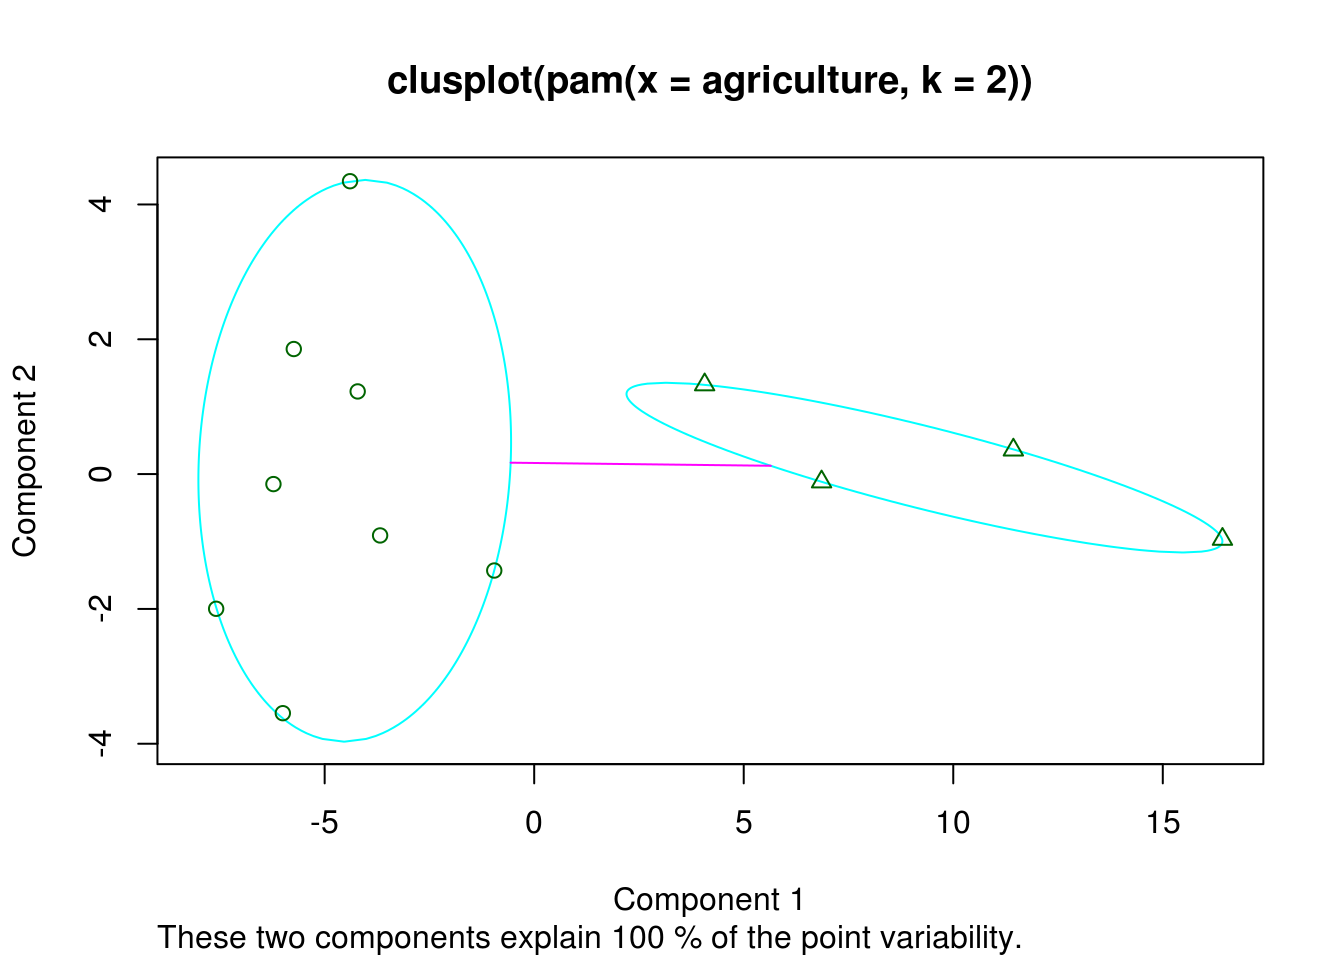
\includegraphics{r-intro-multivar_files/figure-latex/data_agri_exe-1.pdf}

\begin{Shaded}
\begin{Highlighting}[]
\NormalTok{## Gráfico dendograma usando método aglomeração mais próximo}
\NormalTok{## agnes}
\KeywordTok{plot}\NormalTok{(}\KeywordTok{agnes}\NormalTok{(agriculture), }\DataTypeTok{which.plots =} \DecValTok{2}\NormalTok{, }\DataTypeTok{hang =} \NormalTok{-}\DecValTok{1}\NormalTok{)}
\end{Highlighting}
\end{Shaded}

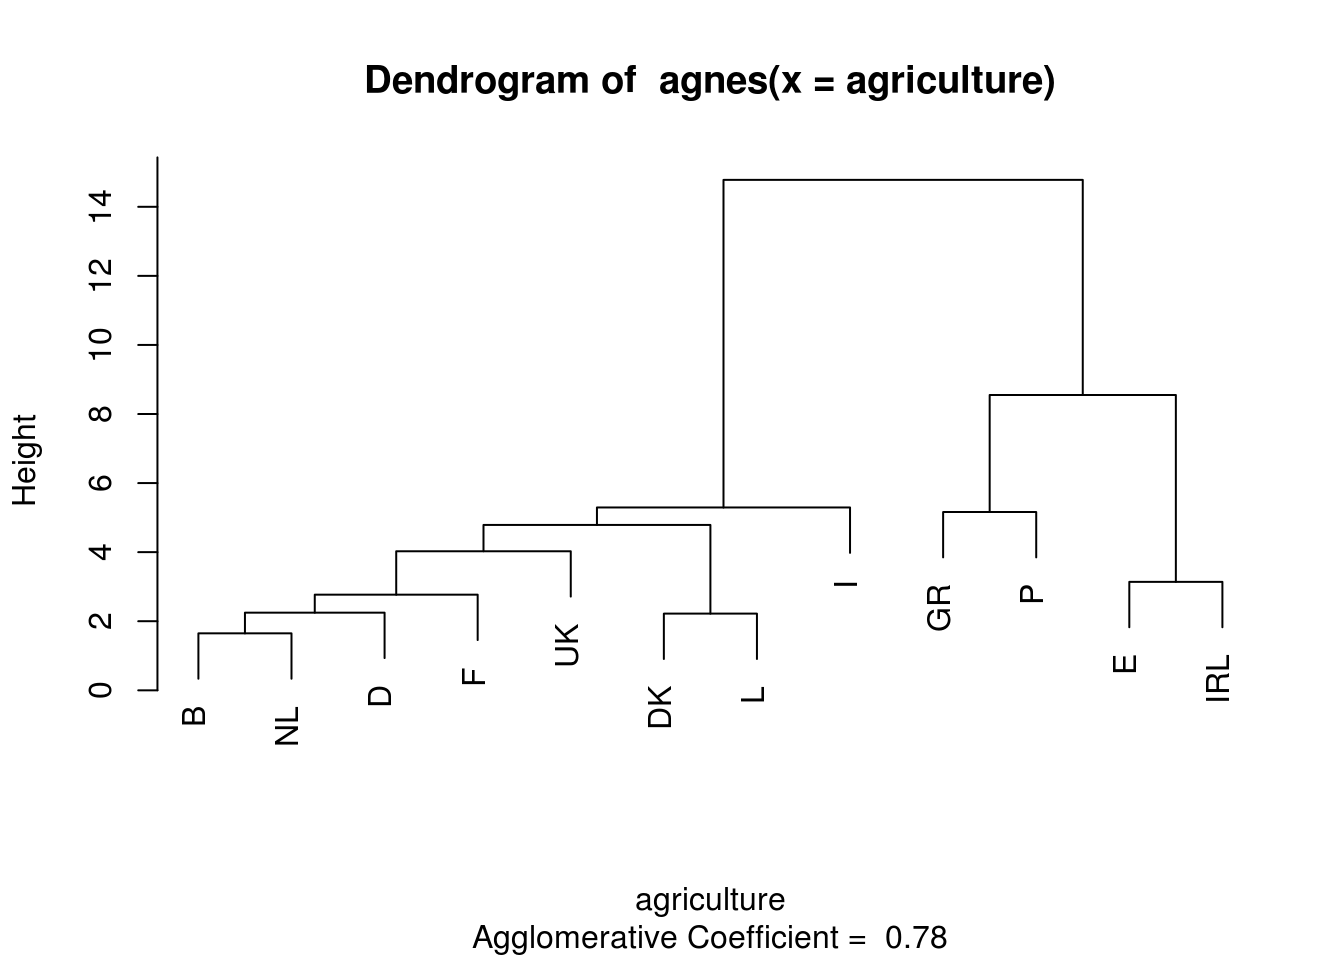
\includegraphics{r-intro-multivar_files/figure-latex/data_agri_exe-2.pdf}

\begin{Shaded}
\begin{Highlighting}[]
\NormalTok{## Plot dissimilaridade usando método divisivo}
\NormalTok{## diana}
\KeywordTok{plot}\NormalTok{(}\KeywordTok{diana}\NormalTok{(agriculture), }\DataTypeTok{which.plots =} \DecValTok{1}\NormalTok{)}
\end{Highlighting}
\end{Shaded}

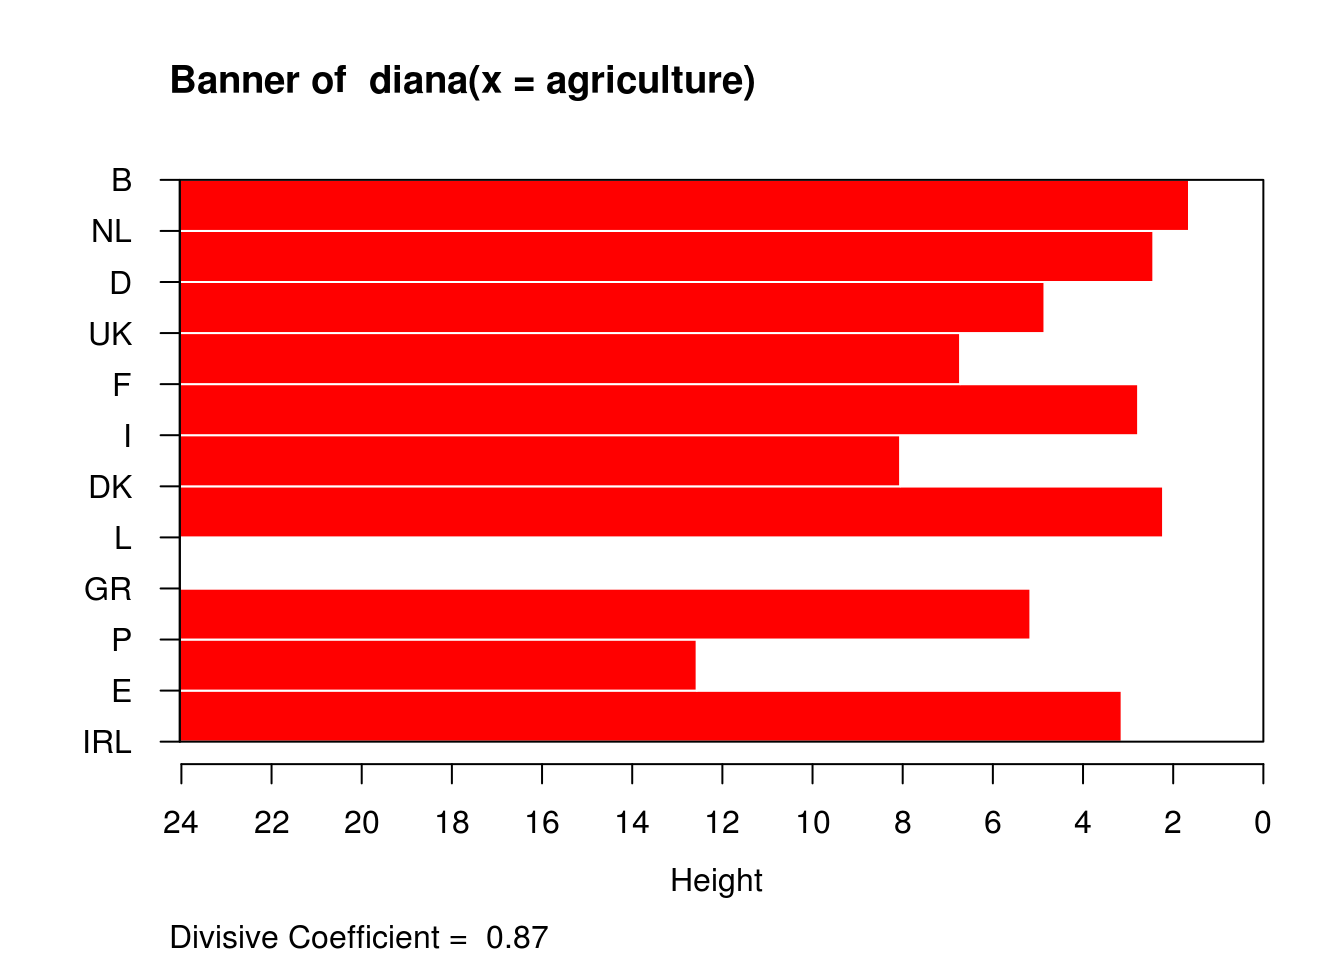
\includegraphics{r-intro-multivar_files/figure-latex/data_agri_exe-3.pdf}

\begin{Shaded}
\begin{Highlighting}[]
\NormalTok{## Usando agnes e diana para conjunto agricultura}
\KeywordTok{par}\NormalTok{(}\DataTypeTok{mfrow=}\KeywordTok{c}\NormalTok{(}\DecValTok{1}\NormalTok{,}\DecValTok{2}\NormalTok{), }\DataTypeTok{mar=}\KeywordTok{c}\NormalTok{(}\DecValTok{3}\NormalTok{,}\DecValTok{2}\NormalTok{,}\DecValTok{2}\NormalTok{,}\DecValTok{0}\NormalTok{))}
\KeywordTok{plot}\NormalTok{(}\KeywordTok{agnes}\NormalTok{(agriculture), }\DataTypeTok{which.plots =} \DecValTok{2}\NormalTok{, }\DataTypeTok{hang =} \NormalTok{-}\DecValTok{1}\NormalTok{,}
     \DataTypeTok{main =} \StringTok{"Método Aglomerativo}\CharTok{\textbackslash{}n}\StringTok{AGNES"}\NormalTok{)}
\KeywordTok{plot}\NormalTok{(}\KeywordTok{diana}\NormalTok{(agriculture), }\DataTypeTok{which.plots =} \DecValTok{2}\NormalTok{, }\DataTypeTok{hang =} \NormalTok{-}\DecValTok{1}\NormalTok{,}
     \DataTypeTok{main =} \StringTok{"Método Divisivo}\CharTok{\textbackslash{}n}\StringTok{DIANA"}\NormalTok{)}
\end{Highlighting}
\end{Shaded}

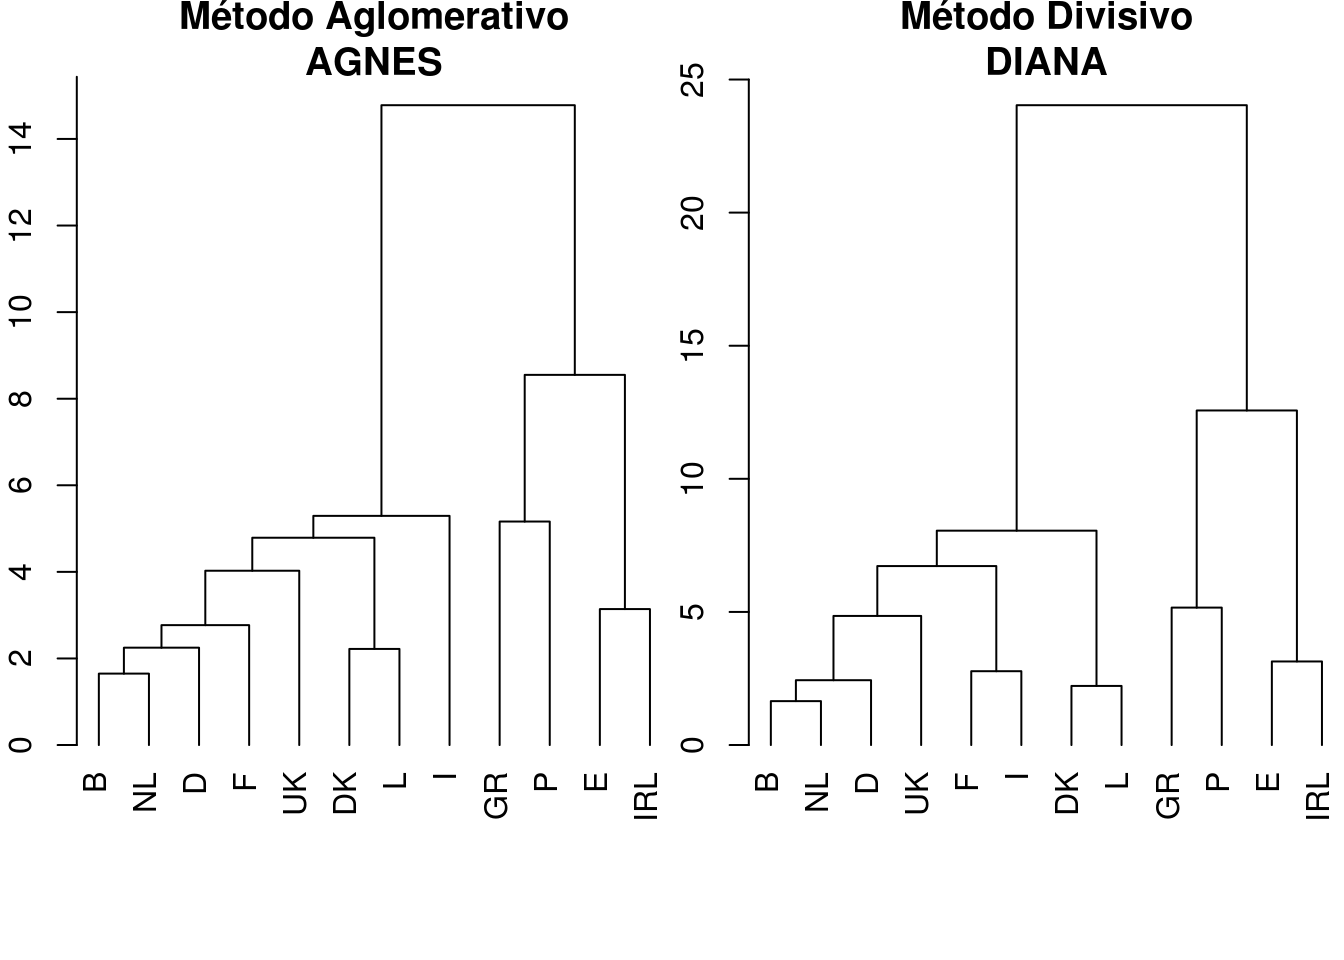
\includegraphics{r-intro-multivar_files/figure-latex/data_agri_exe-4.pdf}

\section{Exemplo cluster USArrest}\label{exemplo-cluster-usarrest}

Neste exemplo vamos utilizar o conjunto USArrest, disponível na
instalação padrão do R.

\begin{Shaded}
\begin{Highlighting}[]
\KeywordTok{data}\NormalTok{(USArrests)}
\CommentTok{#?USArrests}

\NormalTok{d0 =}\StringTok{ }\KeywordTok{dist}\NormalTok{(USArrests) }\CommentTok{# euclidian}
\NormalTok{hc =}\StringTok{ }\KeywordTok{hclust}\NormalTok{(d0, }\StringTok{"average"}\NormalTok{)}
\KeywordTok{plot}\NormalTok{(hc, }\DataTypeTok{hang =} \NormalTok{-}\DecValTok{1}\NormalTok{)}
\CommentTok{# Criar 10 grupos}
\NormalTok{memb =}\StringTok{ }\KeywordTok{cutree}\NormalTok{(hc, }\DataTypeTok{k =} \DecValTok{10}\NormalTok{)}
\CommentTok{# Anota no gráfico os 10 grupos}
\KeywordTok{rect.hclust}\NormalTok{(hc, }\DecValTok{10}\NormalTok{)}
\end{Highlighting}
\end{Shaded}

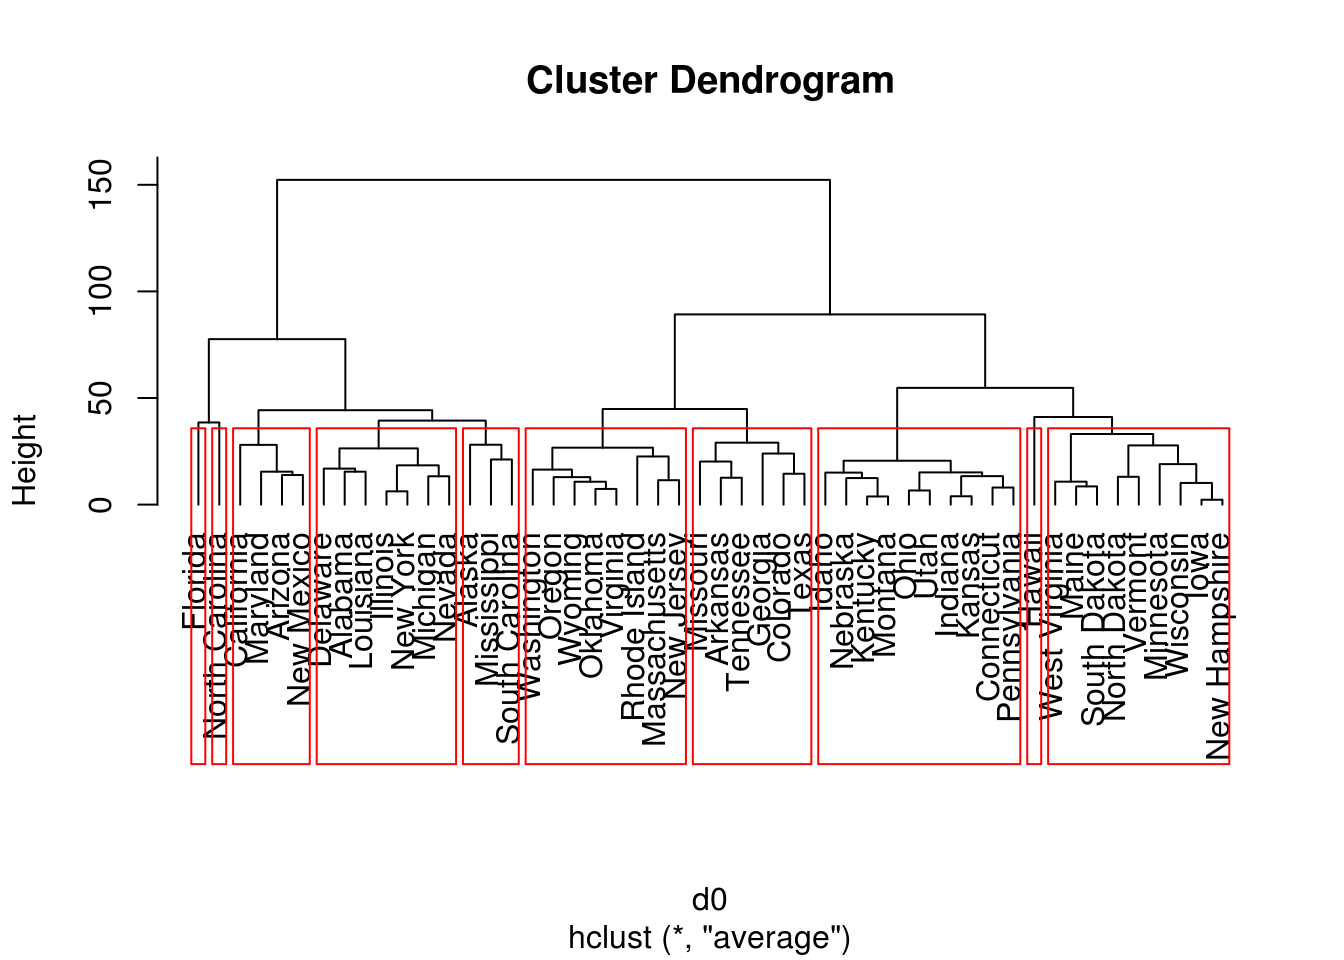
\includegraphics{r-intro-multivar_files/figure-latex/cluArrest-1.pdf}

Como exercício, será trabalhado a seguinte situação: Gostaríamos de
saber quais são os estados que compoem o grupo 1 e qual a média de
assalto (variável \emph{Assault}) para cada grupo.

\begin{Shaded}
\begin{Highlighting}[]
\CommentTok{# Cria conjunto de dados a partir da divisão inicial com}
\CommentTok{# 10 grupos, com as variáveis State e grp10}
\NormalTok{dAssault =}\StringTok{ }\KeywordTok{data.frame}\NormalTok{(}\DataTypeTok{State =} \KeywordTok{names}\NormalTok{(memb), }\DataTypeTok{grp10 =} \NormalTok{memb)}
\CommentTok{# Utilizando a biblioteca dplyr, transformamos o conjunto}
\CommentTok{# dAssault para criar uma nova variável grp3}
\NormalTok{dAssault =}\StringTok{ }\NormalTok{dAssault %>%}\StringTok{ }\KeywordTok{mutate}\NormalTok{(}\DataTypeTok{grp3 =} \KeywordTok{cutree}\NormalTok{(hc, }\DataTypeTok{k =} \DecValTok{3}\NormalTok{), }\DataTypeTok{Assault =} \NormalTok{USArrests$Assault)}
\CommentTok{# calculamos a média por cada grupo grp10}
\NormalTok{dAssault %>%}\StringTok{ }\KeywordTok{group_by}\NormalTok{(grp10) %>%}\StringTok{ }\KeywordTok{summarize}\NormalTok{(}\DataTypeTok{media=}\KeywordTok{mean}\NormalTok{(Assault))}
\end{Highlighting}
\end{Shaded}

\begin{verbatim}
## # A tibble: 10 × 2
##    grp10     media
##    <int>     <dbl>
## 1      1 247.57143
## 2      2 267.00000
## 3      3 288.75000
## 4      4 195.33333
## 5      5 112.40000
## 6      6 335.00000
## 7      7  46.00000
## 8      8  64.55556
## 9      9 156.75000
## 10    10 337.00000
\end{verbatim}

\begin{Shaded}
\begin{Highlighting}[]
\CommentTok{# selecionamos os estados que estão associados ao grupo 1}
\NormalTok{dAssault %>%}\StringTok{ }\KeywordTok{filter}\NormalTok{(grp10 ==}\StringTok{ }\DecValTok{1}\NormalTok{)}
\end{Highlighting}
\end{Shaded}

\begin{verbatim}
##       State grp10 grp3 Assault
## 1   Alabama     1    1     236
## 2  Delaware     1    1     238
## 3  Illinois     1    1     249
## 4 Louisiana     1    1     249
## 5  Michigan     1    1     255
## 6    Nevada     1    1     252
## 7  New York     1    1     254
\end{verbatim}

\begin{Shaded}
\begin{Highlighting}[]
\CommentTok{# calculamos a média e o número de estados por cada grupo grp3}
\NormalTok{dAssault %>%}\StringTok{ }
\StringTok{  }\KeywordTok{group_by}\NormalTok{(grp3) %>%}\StringTok{ }
\StringTok{  }\KeywordTok{summarize}\NormalTok{(}\DataTypeTok{media=}\KeywordTok{mean}\NormalTok{(Assault), }\DataTypeTok{prop =} \KeywordTok{sum}\NormalTok{(Assault)/}\KeywordTok{sum}\NormalTok{(USArrests$Assault),}
            \DataTypeTok{qtd =} \KeywordTok{n}\NormalTok{()) %>%}\StringTok{ }\KeywordTok{arrange}\NormalTok{(prop)}
\end{Highlighting}
\end{Shaded}

\begin{verbatim}
## # A tibble: 3 × 4
##    grp3    media      prop   qtd
##   <int>    <dbl>     <dbl> <int>
## 1     3  87.5500 0.2050832    20
## 2     2 173.2857 0.2841415    14
## 3     1 272.5625 0.5107754    16
\end{verbatim}

Pode-se usa a ANOVA para avaliar o número de grupos, confira o código a
seguir

\begin{Shaded}
\begin{Highlighting}[]
\CommentTok{# ANOVA para grp10}
\NormalTok{aovGrp10 =}\StringTok{ }\KeywordTok{aov}\NormalTok{(Assault ~}\StringTok{ }\KeywordTok{as.factor}\NormalTok{(grp10), }\DataTypeTok{data =} \NormalTok{dAssault)}
\KeywordTok{summary}\NormalTok{(aovGrp10)}
\end{Highlighting}
\end{Shaded}

\begin{verbatim}
##                  Df Sum Sq Mean Sq F value Pr(>F)    
## as.factor(grp10)  9 335715   37302   324.5 <2e-16 ***
## Residuals        40   4598     115                   
## ---
## Signif. codes:  0 '***' 0.001 '**' 0.01 '*' 0.05 '.' 0.1 ' ' 1
\end{verbatim}

\begin{Shaded}
\begin{Highlighting}[]
\CommentTok{# ANOVA para grp3}
\NormalTok{aovGrp3 =}\StringTok{ }\KeywordTok{aov}\NormalTok{(Assault ~}\StringTok{ }\KeywordTok{as.factor}\NormalTok{(grp3), }\DataTypeTok{data =} \NormalTok{dAssault)}
\KeywordTok{summary}\NormalTok{(aovGrp3)}
\end{Highlighting}
\end{Shaded}

\begin{verbatim}
##                 Df Sum Sq Mean Sq F value Pr(>F)    
## as.factor(grp3)  2 304387  152194   199.1 <2e-16 ***
## Residuals       47  35926     764                   
## ---
## Signif. codes:  0 '***' 0.001 '**' 0.01 '*' 0.05 '.' 0.1 ' ' 1
\end{verbatim}

\begin{Shaded}
\begin{Highlighting}[]
\CommentTok{# OBS: todo modelo linear aumenta a explicação com a }
\CommentTok{# adição de novas variáveis ao modelo, faz-se necessário}
\CommentTok{# criar uma penalização para auxiliar na escolha entre modelos}
\CommentTok{# além de definir um critério}
\NormalTok{(}\DataTypeTok{mseGrp10 =} \KeywordTok{sqrt}\NormalTok{(}\KeywordTok{summary}\NormalTok{(aovGrp10)[[}\DecValTok{1}\NormalTok{]]$}\StringTok{`}\DataTypeTok{Mean Sq}\StringTok{`}\NormalTok{[}\DecValTok{2}\NormalTok{]))}
\end{Highlighting}
\end{Shaded}

\begin{verbatim}
## [1] 10.72138
\end{verbatim}

\begin{Shaded}
\begin{Highlighting}[]
\NormalTok{(}\DataTypeTok{mseGrp3 =} \KeywordTok{sqrt}\NormalTok{(}\KeywordTok{summary}\NormalTok{(aovGrp3)[[}\DecValTok{1}\NormalTok{]]$}\StringTok{`}\DataTypeTok{Mean Sq}\StringTok{`}\NormalTok{[}\DecValTok{2}\NormalTok{]))}
\end{Highlighting}
\end{Shaded}

\begin{verbatim}
## [1] 27.64738
\end{verbatim}

\begin{Shaded}
\begin{Highlighting}[]
\CommentTok{# critério mse - log(num fatores)}
\NormalTok{mseGrp10 -}\StringTok{ }\KeywordTok{log}\NormalTok{(}\DecValTok{10}\NormalTok{)}
\end{Highlighting}
\end{Shaded}

\begin{verbatim}
## [1] 8.418795
\end{verbatim}

\begin{Shaded}
\begin{Highlighting}[]
\NormalTok{mseGrp3 -}\StringTok{ }\KeywordTok{log}\NormalTok{(}\DecValTok{3}\NormalTok{)}
\end{Highlighting}
\end{Shaded}

\begin{verbatim}
## [1] 26.54877
\end{verbatim}

Por fim, a apresentação dos grupos, também pode ser feita com a função
\emph{clusplot}

\begin{Shaded}
\begin{Highlighting}[]
\KeywordTok{clusplot}\NormalTok{(USArrests, }\KeywordTok{cutree}\NormalTok{(hc, }\DataTypeTok{k =} \DecValTok{3}\NormalTok{), }\DataTypeTok{shade =} \OtherTok{TRUE}\NormalTok{, }\DataTypeTok{color =} \OtherTok{TRUE}\NormalTok{,}
         \DataTypeTok{col.clus =} \KeywordTok{c}\NormalTok{(}\StringTok{"red"}\NormalTok{, }\StringTok{"grey20"}\NormalTok{, }\StringTok{"blue"}\NormalTok{))}
\end{Highlighting}
\end{Shaded}

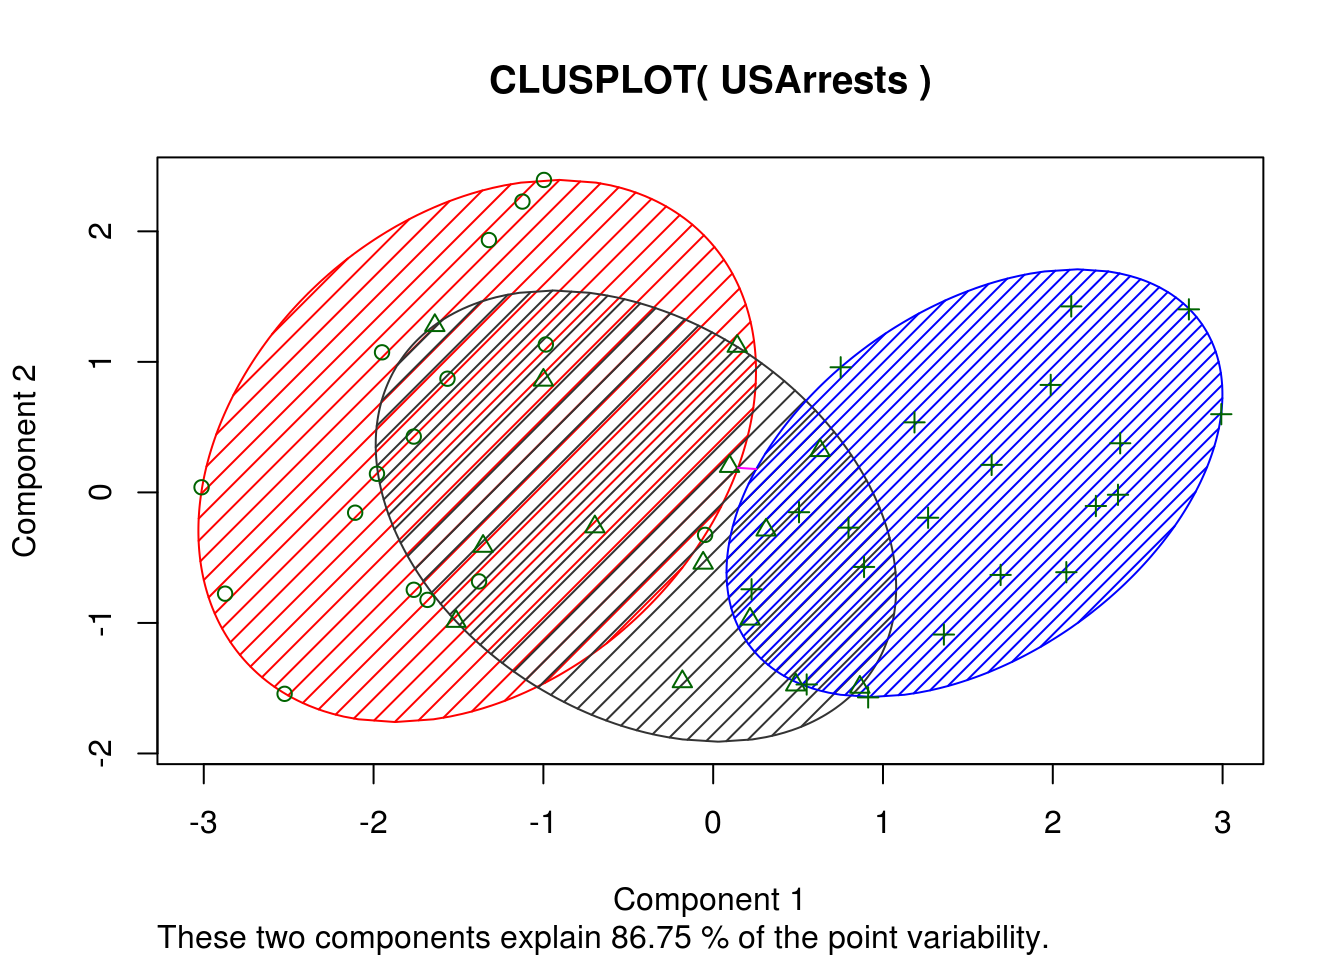
\includegraphics{r-intro-multivar_files/figure-latex/plotGrp3-1.pdf}

\chapter{Análise de Componentes Principais}\label{PCA}

É uma alternativa à Análise Fatorial (FA), apesar dos objetivos serem
semelhantes (PCA e FA), na PCA se busca obter o modelo descritivo dos
dados enquanto na FA se busca o modelo estrutural.

Outro destaque importante é que a matriz/vetor de cargas
\emph{``loadings''} possuírem valores equivalentes, na FA estes são
menores. Isto ocorre porque na PCA é ajustado um modelo para a variância
completa da matriz de correlação das variáveis e na FA o processo é
realizado somente para a variância comum.

Nesta seção serão utilizados as seguinte bibliotecas do R.

\begin{Shaded}
\begin{Highlighting}[]
\KeywordTok{autoLib}\NormalTok{(}\StringTok{'psych'}\NormalTok{)}
\end{Highlighting}
\end{Shaded}

\begin{verbatim}
## Loading required package: psych
\end{verbatim}

\begin{verbatim}
## psych 
##  TRUE
\end{verbatim}

\begin{Shaded}
\begin{Highlighting}[]
\NormalTok{knitr::opts_knit$}\KeywordTok{set}\NormalTok{(}\DataTypeTok{fig.width=}\DecValTok{5}\NormalTok{, }\DataTypeTok{fig.height=}\DecValTok{5}\NormalTok{, }\DataTypeTok{fig.align=}\StringTok{'center'}\NormalTok{)}
\end{Highlighting}
\end{Shaded}

\section{Métodos de cálculo}\label{metodos-de-calculo}

O cálculo de componentes principais pode ser feito, em geral, de duas
formas:

\begin{itemize}
\tightlist
\item
  \emph{princomp} ou \emph{principal(psych)}: Autovalor/Autovetor
\item
  \emph{prcomp}: decomposição SVD
\end{itemize}

A documentação do \emph{R} indica o uso da função prcomp por apresentar
melhor precisão numérica (por causa do método). Já a função
\emph{principal(psych)} apresenta resultados mais detalhados.

De forma geral, o que ocorre é a construção de novas variáveis (fatores)
que são a combinação linear entre as variáveis originais mas apresentam
certas qualidades de interesse, como por exemplo a independência entre
os novos fatores e que estes representam a maior variação possível.

Pode-se dizer que as novas variáveis ou fatores, formam uma rotação (ou
projeção) em um novo conjunto de eixos. As direções são escolhidas com
base na máxima variabilidade observada.

No final do processo, tem-se variáveis independentes entre si e que
explicam uma porção da variação inicial dos dados. Geralmente, 2 ou 3
componentes são suficientes para exlicar mais que \(80\%\) da variação
total.

\section{Exemplo da função prcomp}\label{exemplo-da-funcao-prcomp}

\begin{Shaded}
\begin{Highlighting}[]
\NormalTok{## Variáveis na escala original, inapropriado}
\KeywordTok{prcomp}\NormalTok{(USArrests) }
\end{Highlighting}
\end{Shaded}

\begin{verbatim}
## Standard deviations:
## [1] 83.732400 14.212402  6.489426  2.482790
## 
## Rotation:
##                 PC1         PC2         PC3         PC4
## Murder   0.04170432 -0.04482166  0.07989066 -0.99492173
## Assault  0.99522128 -0.05876003 -0.06756974  0.03893830
## UrbanPop 0.04633575  0.97685748 -0.20054629 -0.05816914
## Rape     0.07515550  0.20071807  0.97408059  0.07232502
\end{verbatim}

\begin{Shaded}
\begin{Highlighting}[]
\NormalTok{## Variáveis trasnformadas para eliminar efeito de diferença}
\NormalTok{## entre escala/medida}
\KeywordTok{prcomp}\NormalTok{(USArrests, }\DataTypeTok{scale =} \OtherTok{TRUE}\NormalTok{)}
\end{Highlighting}
\end{Shaded}

\begin{verbatim}
## Standard deviations:
## [1] 1.5748783 0.9948694 0.5971291 0.4164494
## 
## Rotation:
##                 PC1        PC2        PC3         PC4
## Murder   -0.5358995  0.4181809 -0.3412327  0.64922780
## Assault  -0.5831836  0.1879856 -0.2681484 -0.74340748
## UrbanPop -0.2781909 -0.8728062 -0.3780158  0.13387773
## Rape     -0.5434321 -0.1673186  0.8177779  0.08902432
\end{verbatim}

\begin{Shaded}
\begin{Highlighting}[]
\NormalTok{## é possível escolher apenas algumas variávies de interesse}
\KeywordTok{prcomp}\NormalTok{(~}\StringTok{ }\NormalTok{Murder +}\StringTok{ }\NormalTok{Assault +}\StringTok{ }\NormalTok{Rape, }\DataTypeTok{data =} \NormalTok{USArrests, }\DataTypeTok{scale =} \OtherTok{TRUE}\NormalTok{)}
\end{Highlighting}
\end{Shaded}

\begin{verbatim}
## Standard deviations:
## [1] 1.5357670 0.6767949 0.4282154
## 
## Rotation:
##                PC1        PC2        PC3
## Murder  -0.5826006  0.5339532 -0.6127565
## Assault -0.6079818  0.2140236  0.7645600
## Rape    -0.5393836 -0.8179779 -0.1999436
\end{verbatim}

\begin{Shaded}
\begin{Highlighting}[]
\NormalTok{## gráfico para escolher o número de componentes}
\KeywordTok{screeplot}\NormalTok{(}\KeywordTok{prcomp}\NormalTok{(USArrests, }\DataTypeTok{scale =} \OtherTok{TRUE}\NormalTok{))}
\end{Highlighting}
\end{Shaded}

\begin{center}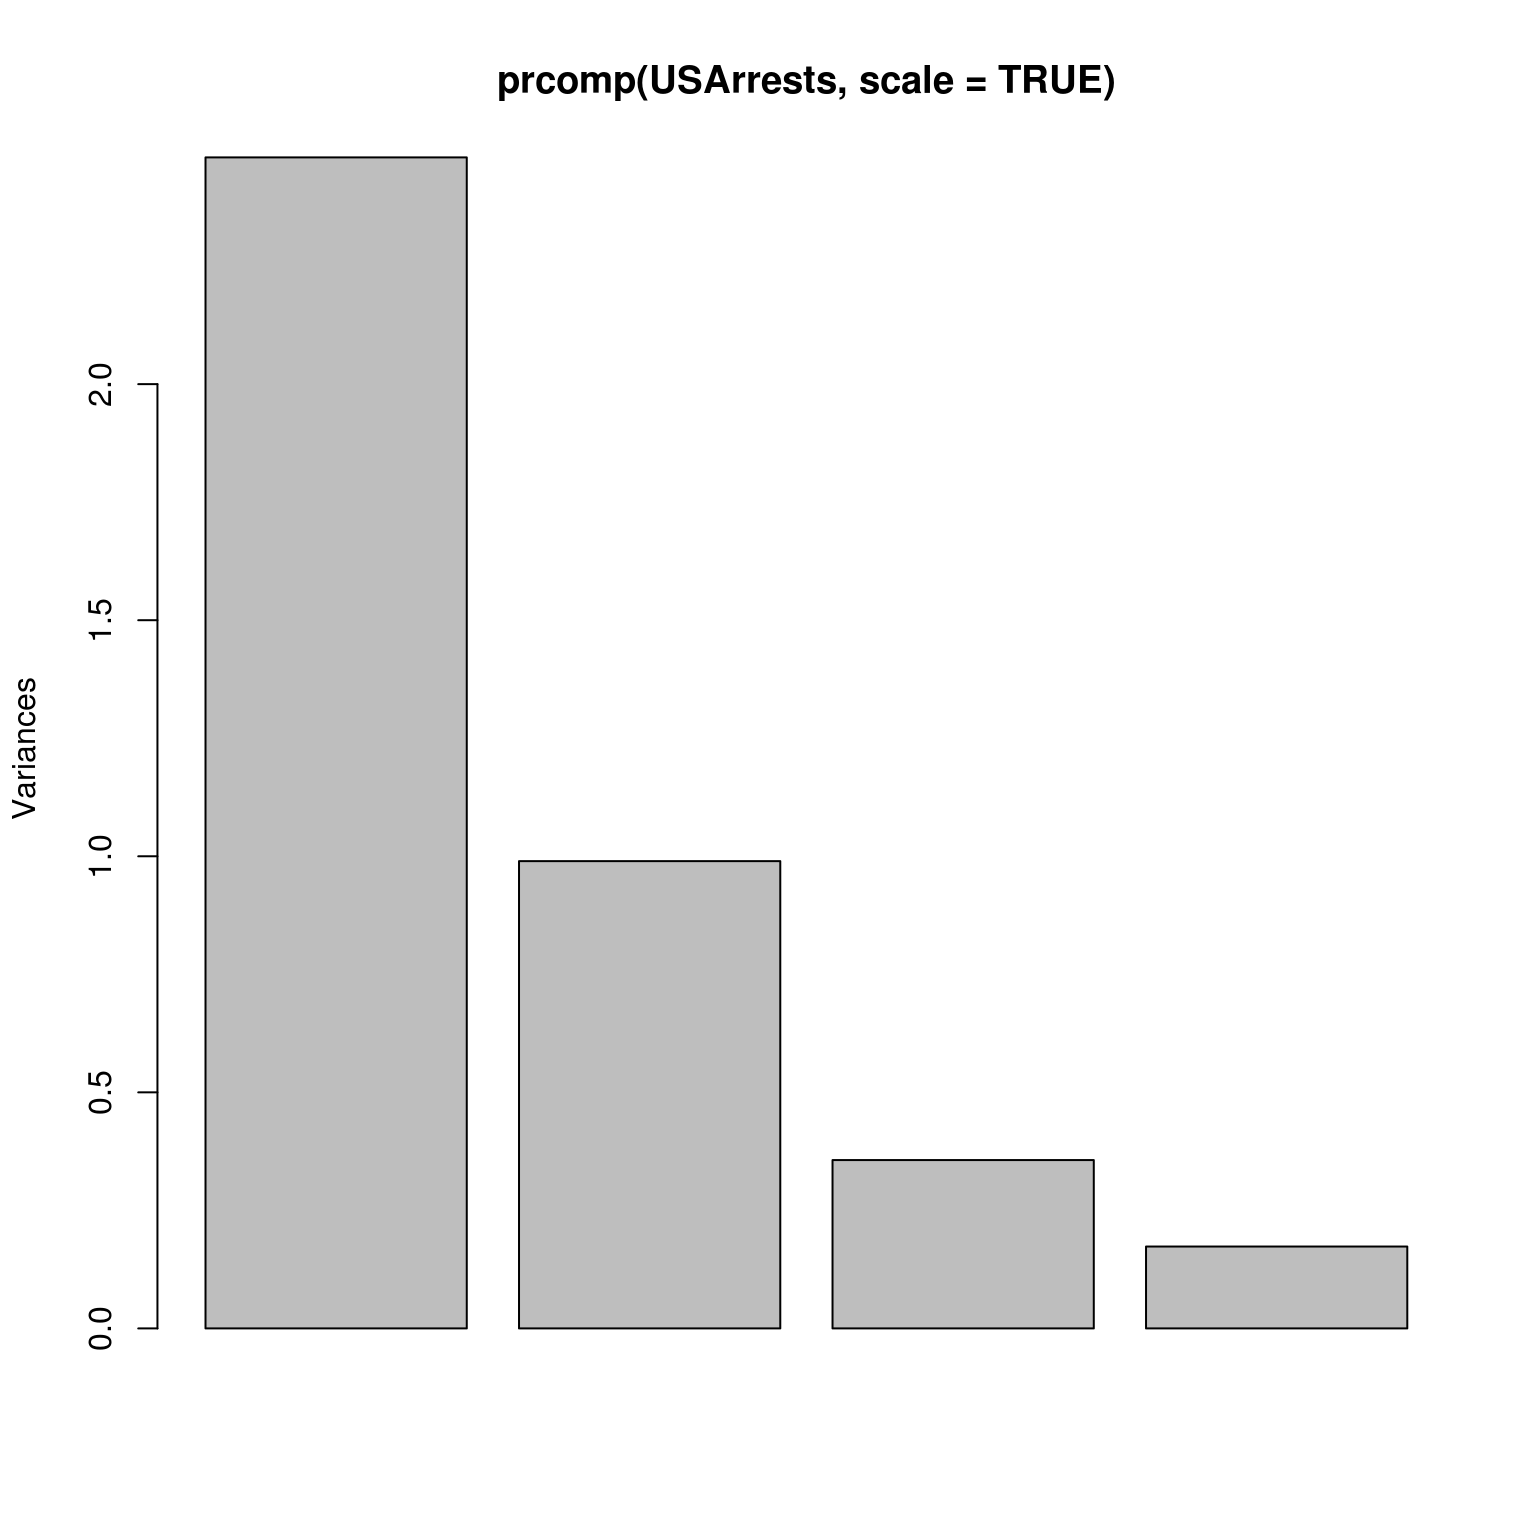
\includegraphics{r-intro-multivar_files/figure-latex/exe_prcomp-1} \end{center}

\begin{Shaded}
\begin{Highlighting}[]
\NormalTok{## outro gráfico com a representação da variância explicada por }
\NormalTok{## cada fator}
\KeywordTok{plot}\NormalTok{(}\KeywordTok{prcomp}\NormalTok{(USArrests))}
\end{Highlighting}
\end{Shaded}

\begin{center}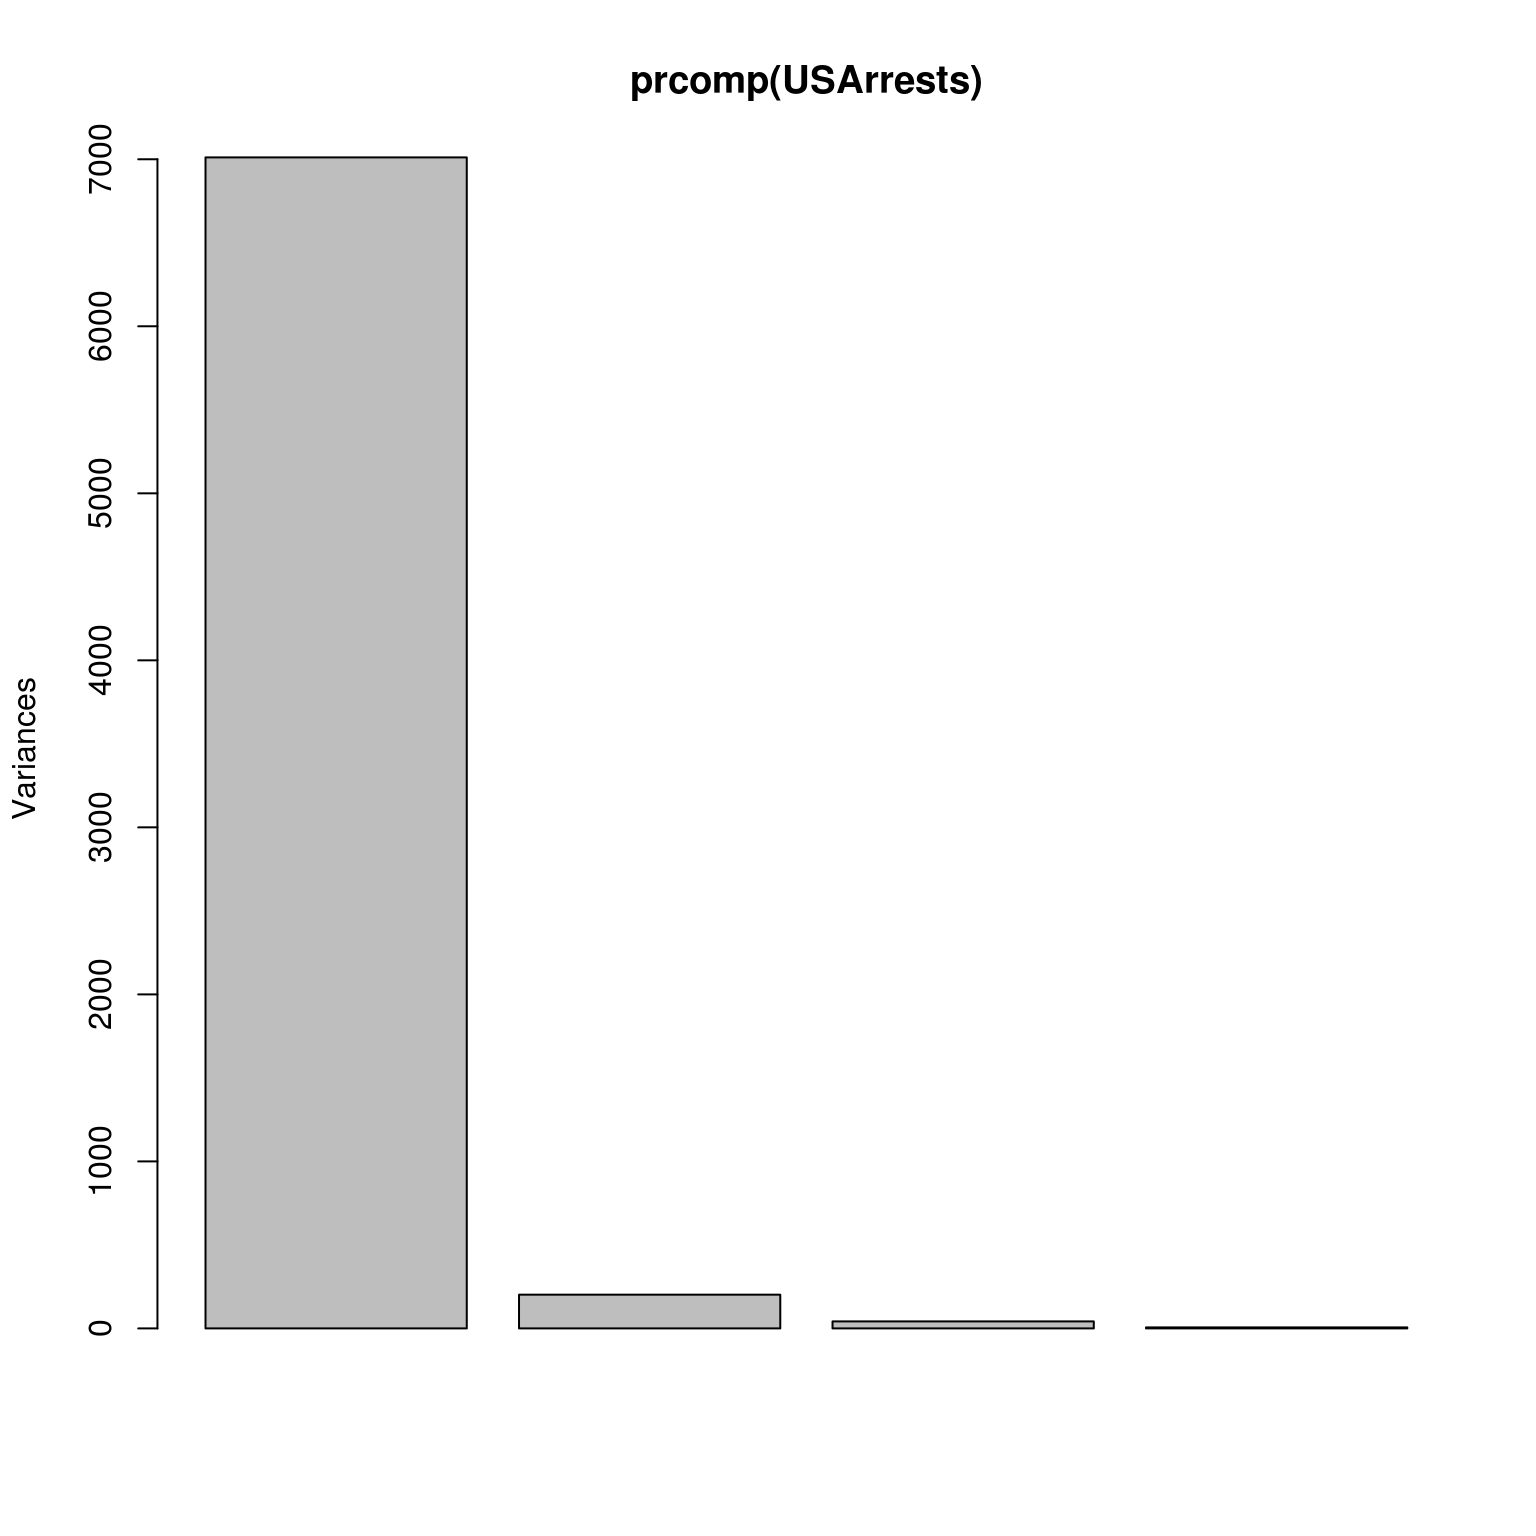
\includegraphics{r-intro-multivar_files/figure-latex/exe_prcomp-2} \end{center}

\begin{Shaded}
\begin{Highlighting}[]
\NormalTok{## sumário com os valores explicados e variância total acumulada}
\KeywordTok{summary}\NormalTok{(}\KeywordTok{prcomp}\NormalTok{(USArrests, }\DataTypeTok{scale =} \OtherTok{TRUE}\NormalTok{))}
\end{Highlighting}
\end{Shaded}

\begin{verbatim}
## Importance of components:
##                           PC1    PC2     PC3     PC4
## Standard deviation     1.5749 0.9949 0.59713 0.41645
## Proportion of Variance 0.6201 0.2474 0.08914 0.04336
## Cumulative Proportion  0.6201 0.8675 0.95664 1.00000
\end{verbatim}

\begin{Shaded}
\begin{Highlighting}[]
\NormalTok{## gráfico biplot}
\KeywordTok{biplot}\NormalTok{(}\KeywordTok{prcomp}\NormalTok{(USArrests, }\DataTypeTok{scale =} \OtherTok{TRUE}\NormalTok{))}
\KeywordTok{abline}\NormalTok{(}\DataTypeTok{v=}\DecValTok{0}\NormalTok{,}\DataTypeTok{h=}\DecValTok{0}\NormalTok{,}\DataTypeTok{col=}\StringTok{"red"}\NormalTok{, }\DataTypeTok{lty=}\DecValTok{2}\NormalTok{)}
\end{Highlighting}
\end{Shaded}

\begin{center}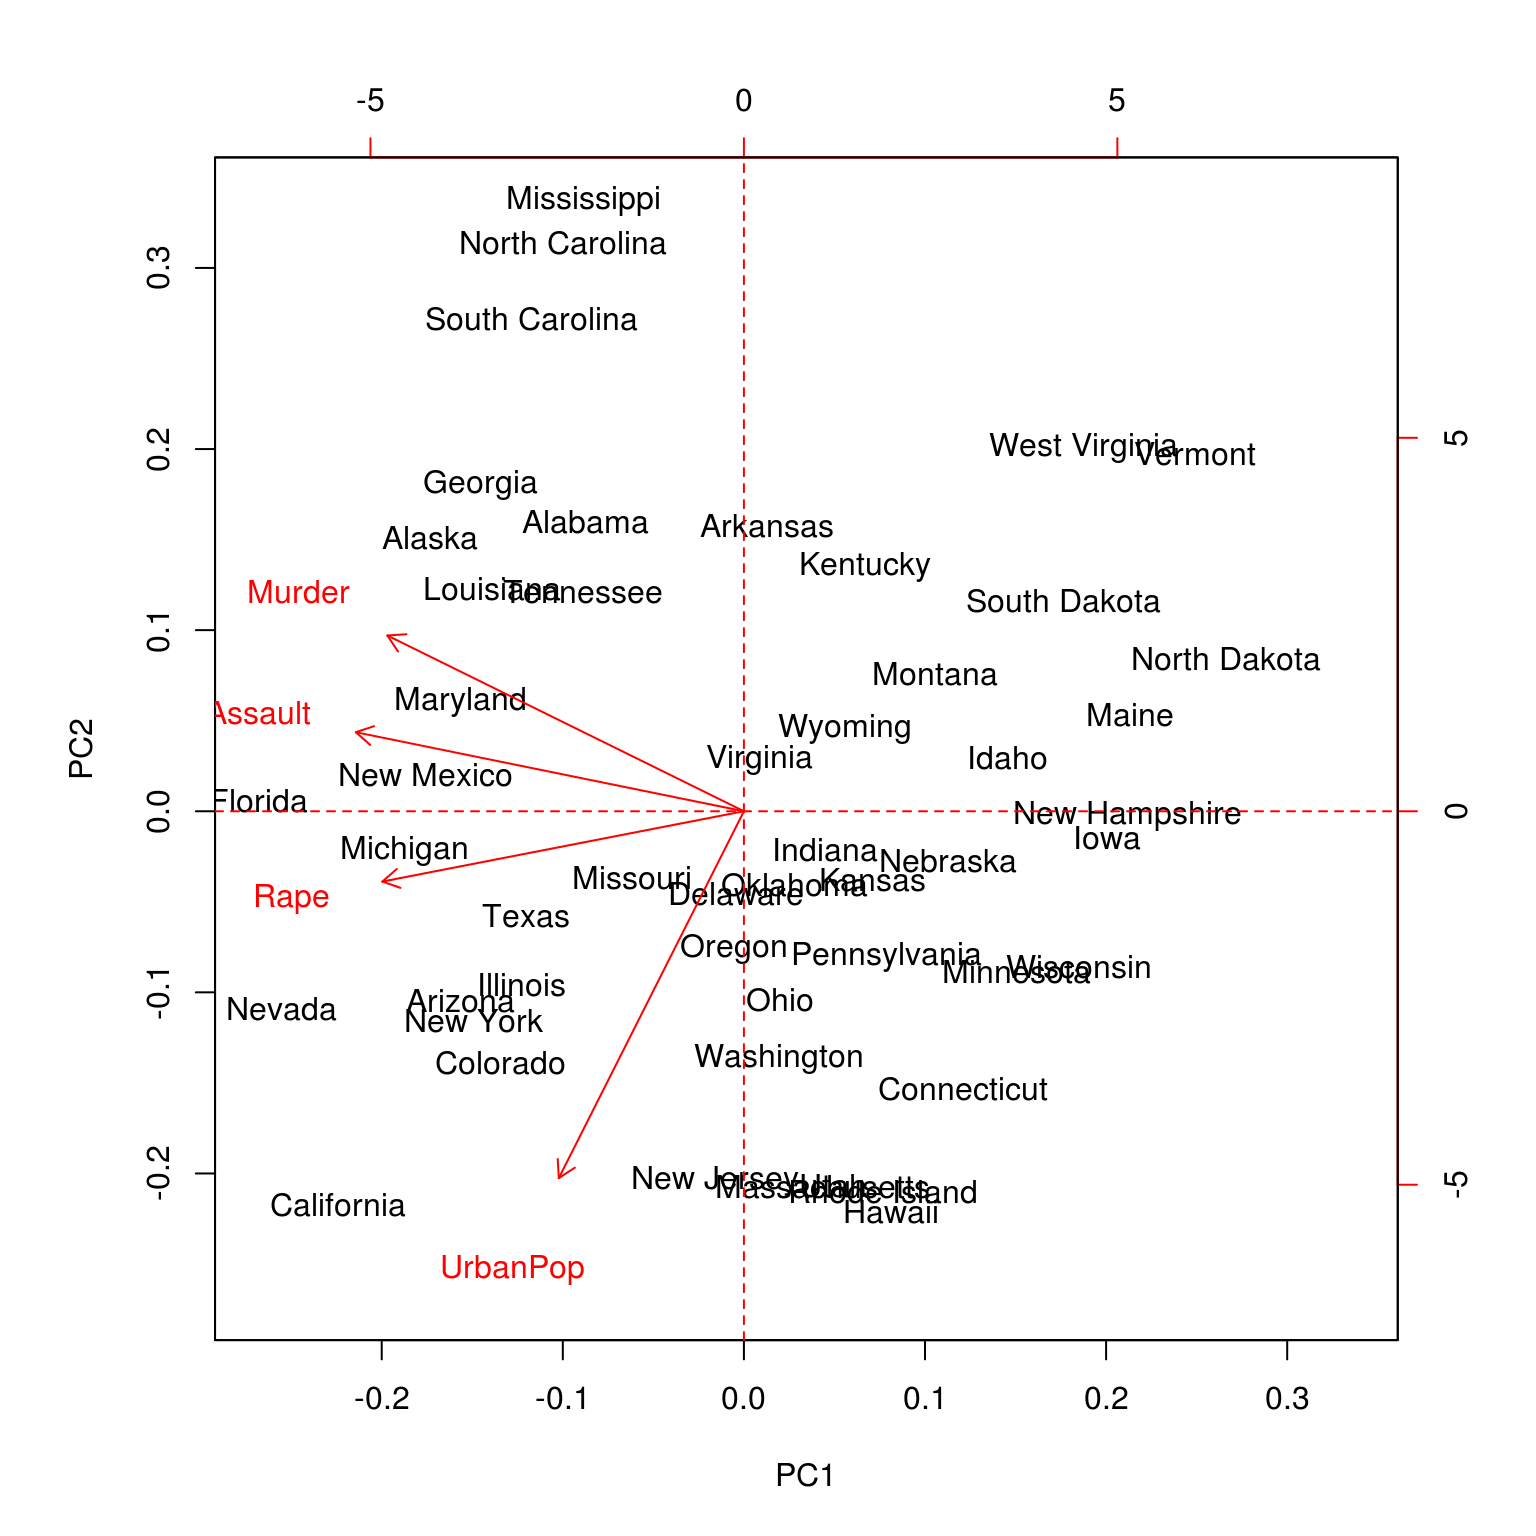
\includegraphics{r-intro-multivar_files/figure-latex/exe_prcomp-3} \end{center}

\section{Exemplo da função principal
(psych)}\label{exemplo-da-funcao-principal-psych}

\begin{Shaded}
\begin{Highlighting}[]
\CommentTok{#Four principal components of the Harman 24 variable problem}
\CommentTok{#compare to a four factor principal axes solution using factor.congruence}
\CommentTok{# Calcula o PCA com rotação varimax}
\NormalTok{pc0 <-}\StringTok{ }\KeywordTok{principal}\NormalTok{(Harman74.cor$cov,}\DecValTok{4}\NormalTok{,}\DataTypeTok{rotate=}\StringTok{"varimax"}\NormalTok{)}
\CommentTok{# Calcula o PCA sem rotação (similar prcomp)}
\NormalTok{pc1 <-}\StringTok{ }\KeywordTok{principal}\NormalTok{(Harman74.cor$cov,}\DecValTok{4}\NormalTok{,}\DataTypeTok{rotate=}\StringTok{"none"}\NormalTok{)}
\CommentTok{# resultado do pc0}
\KeywordTok{print}\NormalTok{(pc0)}
\end{Highlighting}
\end{Shaded}

\begin{verbatim}
## Principal Components Analysis
## Call: principal(r = Harman74.cor$cov, nfactors = 4, rotate = "varimax")
## Standardized loadings (pattern matrix) based upon correlation matrix
##                          RC1   RC3   RC2  RC4   h2   u2 com
## VisualPerception        0.16  0.71  0.23 0.14 0.60 0.40 1.4
## Cubes                   0.09  0.59  0.08 0.03 0.37 0.63 1.1
## PaperFormBoard          0.14  0.66 -0.04 0.11 0.47 0.53 1.2
## Flags                   0.25  0.62  0.09 0.03 0.45 0.55 1.4
## GeneralInformation      0.79  0.15  0.22 0.11 0.70 0.30 1.3
## PargraphComprehension   0.81  0.18  0.07 0.21 0.73 0.27 1.2
## SentenceCompletion      0.85  0.15  0.15 0.06 0.77 0.23 1.1
## WordClassification      0.64  0.31  0.24 0.11 0.57 0.43 1.8
## WordMeaning             0.84  0.16  0.06 0.19 0.78 0.22 1.2
## Addition                0.18 -0.13  0.83 0.12 0.76 0.24 1.2
## Code                    0.18  0.05  0.63 0.37 0.57 0.43 1.8
## CountingDots            0.02  0.17  0.80 0.05 0.67 0.33 1.1
## StraightCurvedCapitals  0.18  0.41  0.62 0.03 0.59 0.41 1.9
## WordRecognition         0.23 -0.01  0.06 0.68 0.52 0.48 1.2
## NumberRecognition       0.12  0.08  0.05 0.67 0.48 0.52 1.1
## FigureRecognition       0.06  0.46  0.05 0.58 0.55 0.45 1.9
## ObjectNumber            0.14  0.01  0.24 0.68 0.54 0.46 1.4
## NumberFigure           -0.02  0.32  0.40 0.50 0.51 0.49 2.7
## FigureWord              0.14  0.25  0.20 0.42 0.30 0.70 2.4
## Deduction               0.43  0.43  0.09 0.30 0.47 0.53 2.8
## NumericalPuzzles        0.18  0.42  0.50 0.17 0.49 0.51 2.5
## ProblemReasoning        0.42  0.41  0.13 0.29 0.45 0.55 3.0
## SeriesCompletion        0.42  0.52  0.25 0.20 0.55 0.45 2.7
## ArithmeticProblems      0.40  0.14  0.55 0.26 0.55 0.45 2.5
## 
##                        RC1  RC3  RC2  RC4
## SS loadings           4.16 3.31 3.22 2.74
## Proportion Var        0.17 0.14 0.13 0.11
## Cumulative Var        0.17 0.31 0.45 0.56
## Proportion Explained  0.31 0.25 0.24 0.20
## Cumulative Proportion 0.31 0.56 0.80 1.00
## 
## Mean item complexity =  1.7
## Test of the hypothesis that 4 components are sufficient.
## 
## The root mean square of the residuals (RMSR) is  0.06 
## 
## Fit based upon off diagonal values = 0.97
\end{verbatim}

\begin{Shaded}
\begin{Highlighting}[]
\CommentTok{# resultado do pc1}
\KeywordTok{print}\NormalTok{(pc1)}
\end{Highlighting}
\end{Shaded}

\begin{verbatim}
## Principal Components Analysis
## Call: principal(r = Harman74.cor$cov, nfactors = 4, rotate = "none")
## Standardized loadings (pattern matrix) based upon correlation matrix
##                         PC1   PC2   PC3   PC4   h2   u2 com
## VisualPerception       0.62 -0.01  0.43 -0.20 0.60 0.40 2.0
## Cubes                  0.40 -0.08  0.40 -0.20 0.37 0.63 2.5
## PaperFormBoard         0.44 -0.19  0.48 -0.11 0.47 0.53 2.4
## Flags                  0.51 -0.18  0.33 -0.22 0.45 0.55 2.4
## GeneralInformation     0.69 -0.32 -0.34 -0.05 0.70 0.30 1.9
## PargraphComprehension  0.69 -0.42 -0.27  0.08 0.73 0.27 2.0
## SentenceCompletion     0.68 -0.42 -0.36 -0.07 0.77 0.23 2.3
## WordClassification     0.69 -0.24 -0.14 -0.12 0.57 0.43 1.4
## WordMeaning            0.69 -0.45 -0.29  0.08 0.78 0.22 2.1
## Addition               0.47  0.54 -0.45 -0.20 0.76 0.24 3.2
## Code                   0.58  0.43 -0.21  0.03 0.57 0.43 2.2
## CountingDots           0.48  0.55 -0.13 -0.34 0.67 0.33 2.8
## StraightCurvedCapitals 0.62  0.28  0.04 -0.37 0.59 0.41 2.1
## WordRecognition        0.45  0.09 -0.06  0.56 0.52 0.48 2.0
## NumberRecognition      0.42  0.14  0.08  0.53 0.48 0.52 2.1
## FigureRecognition      0.53  0.09  0.39  0.33 0.55 0.45 2.6
## ObjectNumber           0.49  0.28 -0.05  0.47 0.54 0.46 2.6
## NumberFigure           0.54  0.39  0.20  0.15 0.51 0.49 2.3
## FigureWord             0.48  0.14  0.12  0.19 0.30 0.70 1.7
## Deduction              0.64 -0.19  0.13  0.07 0.47 0.53 1.3
## NumericalPuzzles       0.62  0.23  0.10 -0.20 0.49 0.51 1.6
## ProblemReasoning       0.64 -0.15  0.11  0.06 0.45 0.55 1.2
## SeriesCompletion       0.71 -0.10  0.15 -0.10 0.55 0.45 1.2
## ArithmeticProblems     0.67  0.20 -0.23 -0.06 0.55 0.45 1.4
## 
##                        PC1  PC2  PC3  PC4
## SS loadings           8.14 2.10 1.69 1.50
## Proportion Var        0.34 0.09 0.07 0.06
## Cumulative Var        0.34 0.43 0.50 0.56
## Proportion Explained  0.61 0.16 0.13 0.11
## Cumulative Proportion 0.61 0.76 0.89 1.00
## 
## Mean item complexity =  2.1
## Test of the hypothesis that 4 components are sufficient.
## 
## The root mean square of the residuals (RMSR) is  0.06 
## 
## Fit based upon off diagonal values = 0.97
\end{verbatim}

\begin{Shaded}
\begin{Highlighting}[]
\CommentTok{# Calcula PCA para conjunto Harman.5, 2 fatores e rotação varimax}
\NormalTok{pc2 <-}\StringTok{ }\KeywordTok{principal}\NormalTok{(Harman}\FloatTok{.5}\NormalTok{,}\DecValTok{2}\NormalTok{,}\DataTypeTok{rotate=}\StringTok{"varimax"}\NormalTok{)}
\NormalTok{pc2}
\end{Highlighting}
\end{Shaded}

\begin{verbatim}
## Principal Components Analysis
## Call: principal(r = Harman.5, nfactors = 2, rotate = "varimax")
## Standardized loadings (pattern matrix) based upon correlation matrix
##               RC1   RC2   h2    u2 com
## population   0.02  0.99 0.99 0.012 1.0
## schooling    0.94 -0.01 0.89 0.115 1.0
## employment   0.14  0.98 0.98 0.021 1.0
## professional 0.83  0.45 0.88 0.120 1.5
## housevalue   0.97 -0.01 0.94 0.062 1.0
## 
##                        RC1  RC2
## SS loadings           2.52 2.15
## Proportion Var        0.50 0.43
## Cumulative Var        0.50 0.93
## Proportion Explained  0.54 0.46
## Cumulative Proportion 0.54 1.00
## 
## Mean item complexity =  1.1
## Test of the hypothesis that 2 components are sufficient.
## 
## The root mean square of the residuals (RMSR) is  0.03 
##  with the empirical chi square  0.29  with prob <  0.59 
## 
## Fit based upon off diagonal values = 1
\end{verbatim}

\begin{Shaded}
\begin{Highlighting}[]
\CommentTok{# compare these correlations to the loadings }
\CommentTok{#  do it for unstandardized scores, and transform obliquely}
\KeywordTok{round}\NormalTok{(}\KeywordTok{cor}\NormalTok{(Harman}\FloatTok{.5}\NormalTok{,pc2$scores),}\DecValTok{2}\NormalTok{)  }
\end{Highlighting}
\end{Shaded}

\begin{verbatim}
##               RC1   RC2
## population   0.02  0.99
## schooling    0.94 -0.01
## employment   0.14  0.98
## professional 0.83  0.45
## housevalue   0.97 -0.01
\end{verbatim}

\begin{Shaded}
\begin{Highlighting}[]
\NormalTok{pc2o <-}\StringTok{ }\KeywordTok{principal}\NormalTok{(Harman}\FloatTok{.5}\NormalTok{,}\DecValTok{2}\NormalTok{,}\DataTypeTok{rotate=}\StringTok{"promax"}\NormalTok{,}\DataTypeTok{covar=}\OtherTok{TRUE}\NormalTok{)}
\NormalTok{pc2o}
\end{Highlighting}
\end{Shaded}

\begin{verbatim}
## Principal Components Analysis
## Call: principal(r = Harman.5, nfactors = 2, rotate = "promax", covar = TRUE)
## Unstandardized loadings (pattern matrix) based upon covariance matrix
##                 RC1     RC2      h2      u2   H2      U2
## population    -40.1 3440.30 1.2e+07 6.7e+03 1.00 5.7e-04
## schooling       1.5   -0.01 2.4e+00 8.1e-01 0.75 2.5e-01
## employment    110.3 1210.10 1.5e+06 5.4e+04 0.96 3.5e-02
## professional   87.7   48.30 1.0e+04 2.9e+03 0.78 2.2e-01
## housevalue   6368.4  -23.16 4.1e+07 2.2e+01 1.00 5.4e-07
## 
##                               RC1         RC2
## SS loadings           40571924.73 13297286.79
## Proportion Var               0.75        0.25
## Cumulative Var               0.75        1.00
## Proportion Explained         0.75        0.25
## Cumulative Proportion        0.75        1.00
## 
##  Standardized loadings (pattern matrix)
##              item   RC1   RC2   h2      u2
## population      1 -0.01  1.00 1.00 5.7e-04
## schooling       2  0.86 -0.01 0.75 2.5e-01
## employment      3  0.09  0.97 0.96 3.5e-02
## professional    4  0.76  0.42 0.78 2.2e-01
## housevalue      5  1.00  0.00 1.00 5.4e-07
## 
##                  RC1  RC2
## SS loadings     3.76 1.23
## Proportion Var  0.75 0.25
## Cumulative Var  0.75 1.00
## Cum. factor Var 0.75 1.00
## 
##  With component correlations of 
##      RC1  RC2
## RC1 1.00 0.04
## RC2 0.04 1.00
## 
## Mean item complexity =  1.1
## Test of the hypothesis that 2 components are sufficient.
## 
## The root mean square of the residuals (RMSR) is  6040.31 
##  with the empirical chi square  8756488842  with prob <  0 
## 
## Fit based upon off diagonal values = 1
\end{verbatim}

\begin{Shaded}
\begin{Highlighting}[]
\KeywordTok{round}\NormalTok{(}\KeywordTok{cov}\NormalTok{(Harman}\FloatTok{.5}\NormalTok{,pc2o$scores),}\DecValTok{2}\NormalTok{) }
\end{Highlighting}
\end{Shaded}

\begin{verbatim}
##                  RC1     RC2
## population     89.53 3438.79
## schooling       1.54    0.05
## employment    155.90 1214.25
## professional   89.56   51.60
## housevalue   6367.49  216.72
\end{verbatim}

\begin{Shaded}
\begin{Highlighting}[]
\NormalTok{pc2o$Structure    }\CommentTok{#this matches the covariances with the scores}
\end{Highlighting}
\end{Shaded}

\begin{verbatim}
##                      RC1          RC2
## population     89.532324 3.438787e+03
## schooling       1.542246 4.714838e-02
## employment    155.900367 1.214255e+03
## professional   89.559504 5.160112e+01
## housevalue   6367.487506 2.167238e+02
\end{verbatim}

\begin{Shaded}
\begin{Highlighting}[]
\KeywordTok{biplot}\NormalTok{(pc2,}\DataTypeTok{main=}\StringTok{"Biplot of the Harman.5 socio-economic variables"}\NormalTok{,}\DataTypeTok{labels=}\KeywordTok{paste0}\NormalTok{(}\DecValTok{1}\NormalTok{:}\DecValTok{12}\NormalTok{))}
\end{Highlighting}
\end{Shaded}

\begin{center}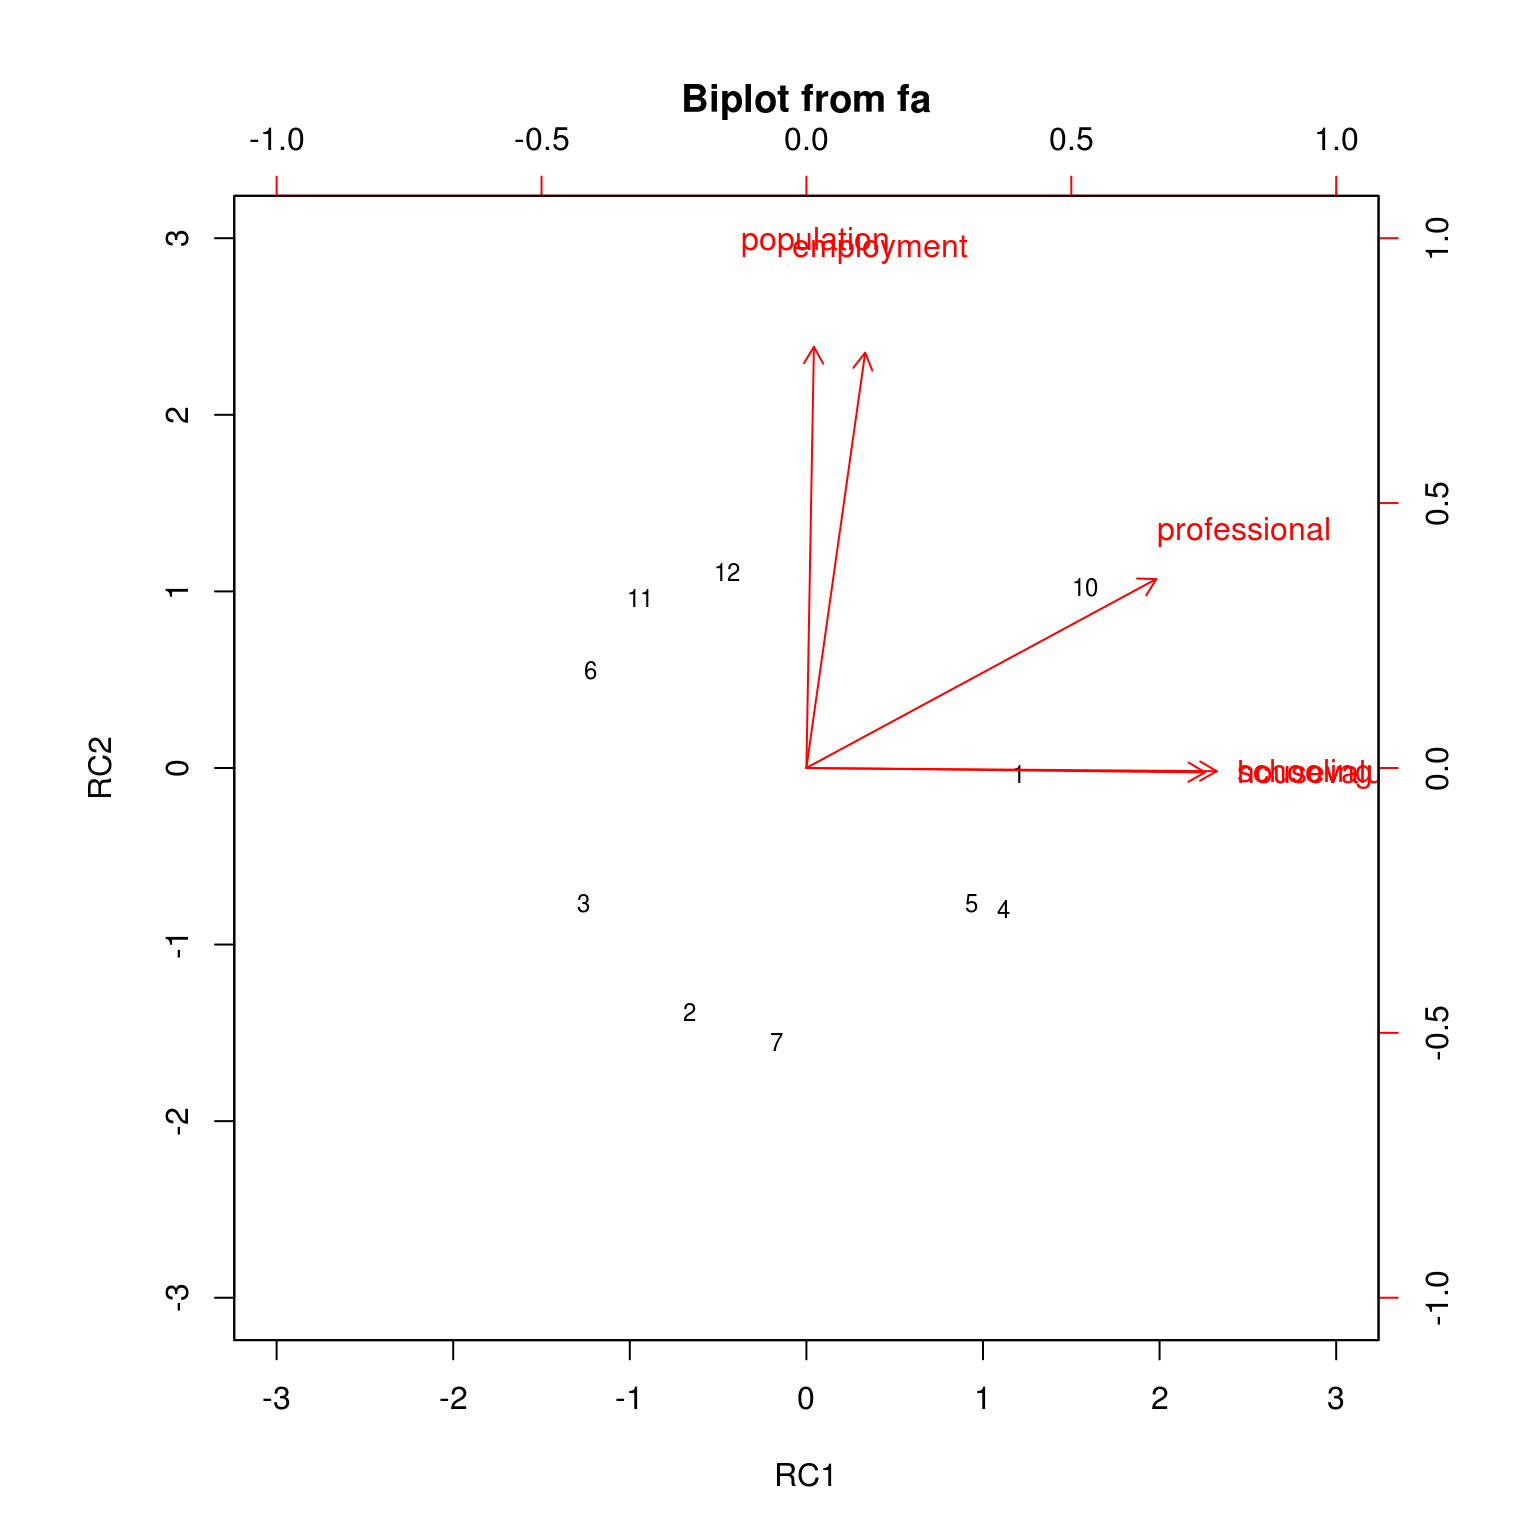
\includegraphics{r-intro-multivar_files/figure-latex/exe_principal-1} \end{center}

\chapter{Análise de Fatores}\label{FA}

O objetivo principal da Análise de Fatores (FA) é identificar um número
reduzido de variáveis latentes ou constructos que explicam os dados
observados ou sob estudo.

No caso de redução da dimensão o problema (PCA \ref{PCA} ou CA \ref{CA})
pode ser resolvido pelo método SVD da matriz de dados original, mas a
solução mais comum é a utilização de PCA ou FA da matriz de covariância
ou correlação.

\section{\texorpdfstring{Algorítmos disponíveis na biblioteca
\emph{psych}}{Algorítmos disponíveis na biblioteca psych}}\label{algoritmos-disponiveis-na-biblioteca-psych}

Ao todo, temos disponível 5 algorítimos para uso com FA na biblioteca
\emph{psych} por meio do comando fa, são eles:

\begin{itemize}
\tightlist
\item
  \emph{minres}: resíduo mínimo
\item
  \emph{principal axis}: utiliza sucessivas decomposições dos
  autovalores na matriz de correlação
\item
  \emph{weighted least squares}: mínimos quadrado ponderados
\item
  \emph{generalized least squares}: mínimos quadrados genrealizados
\item
  \emph{maximum likelihood}: máxima verossimilhança
\end{itemize}

\section{\texorpdfstring{Métodos de rotação
(\emph{psych})}{Métodos de rotação (psych)}}\label{metodos-de-rotacao-psych}

Referente a forma ou método de rotação temos as opções a seguir:

\begin{itemize}
\tightlist
\item
  \emph{ortogonais}: ``none'', ``varimax'', ``quartimax'', ``bentlerT'',
  ``equamax'', ``varimin'', ``geominT'' e ``bifactor''
\item
  \emph{oblíquas}: ``promax'', ``oblimin'', ``simplimax'',
  ``bentlerQ,''geominQ``,''biquartimin" e ``cluster''
\end{itemize}

\section{Exemplo utilizando dataset Harman 24 e comparando com
PCA}\label{exemplo-utilizando-dataset-harman-24-e-comparando-com-pca}

\begin{Shaded}
\begin{Highlighting}[]
\CommentTok{#using the Harman 24 mental tests, compare a principal factor with a principal components solution}
\NormalTok{pc <-}\StringTok{ }\KeywordTok{principal}\NormalTok{(Harman74.cor$cov,}\DecValTok{4}\NormalTok{,}\DataTypeTok{rotate=}\StringTok{"varimax"}\NormalTok{)   }\CommentTok{#principal components}
\NormalTok{pa <-}\StringTok{ }\KeywordTok{fa}\NormalTok{(Harman74.cor$cov,}\DecValTok{4}\NormalTok{,}\DataTypeTok{fm=}\StringTok{"pa"} \NormalTok{,}\DataTypeTok{rotate=}\StringTok{"varimax"}\NormalTok{)  }\CommentTok{#principal axis }
\NormalTok{uls <-}\StringTok{ }\KeywordTok{fa}\NormalTok{(Harman74.cor$cov,}\DecValTok{4}\NormalTok{,}\DataTypeTok{rotate=}\StringTok{"varimax"}\NormalTok{)          }\CommentTok{#unweighted least squares is minres}
\NormalTok{wls <-}\StringTok{ }\KeywordTok{fa}\NormalTok{(Harman74.cor$cov,}\DecValTok{4}\NormalTok{,}\DataTypeTok{fm=}\StringTok{"wls"}\NormalTok{)       }\CommentTok{#weighted least squares}
\end{Highlighting}
\end{Shaded}

\begin{verbatim}
## Loading required namespace: GPArotation
\end{verbatim}

\begin{Shaded}
\begin{Highlighting}[]
\CommentTok{#to show the loadings sorted by absolute value}
\KeywordTok{print}\NormalTok{(uls,}\DataTypeTok{sort=}\OtherTok{TRUE}\NormalTok{)}
\end{Highlighting}
\end{Shaded}

\begin{verbatim}
## Factor Analysis using method =  minres
## Call: fa(r = Harman74.cor$cov, nfactors = 4, rotate = "varimax")
## Standardized loadings (pattern matrix) based upon correlation matrix
##                        item  MR1   MR3   MR2  MR4   h2   u2 com
## WordMeaning               9 0.81  0.20  0.04 0.23 0.74 0.26 1.3
## SentenceCompletion        7 0.81  0.20  0.15 0.07 0.72 0.28 1.2
## PargraphComprehension     6 0.77  0.20  0.07 0.23 0.69 0.31 1.4
## GeneralInformation        5 0.74  0.19  0.21 0.15 0.65 0.35 1.4
## WordClassification        8 0.57  0.34  0.24 0.13 0.51 0.49 2.2
## VisualPerception          1 0.16  0.69  0.19 0.16 0.56 0.44 1.4
## PaperFormBoard            3 0.14  0.57 -0.02 0.11 0.36 0.64 1.2
## Flags                     4 0.23  0.53  0.10 0.08 0.35 0.65 1.5
## SeriesCompletion         23 0.37  0.50  0.24 0.24 0.50 0.50 2.9
## Cubes                     2 0.12  0.44  0.08 0.10 0.22 0.78 1.3
## Deduction                20 0.38  0.40  0.12 0.30 0.41 0.59 3.0
## ProblemReasoning         22 0.37  0.40  0.12 0.30 0.40 0.60 3.1
## Addition                 10 0.17 -0.12  0.83 0.17 0.76 0.24 1.2
## CountingDots             12 0.02  0.21  0.72 0.09 0.56 0.44 1.2
## StraightCurvedCapitals   13 0.19  0.44  0.53 0.08 0.51 0.49 2.3
## Code                     11 0.18  0.12  0.51 0.37 0.45 0.55 2.2
## ArithmeticProblems       24 0.37  0.16  0.50 0.30 0.50 0.50 2.8
## NumericalPuzzles         21 0.17  0.38  0.44 0.22 0.42 0.58 2.8
## ObjectNumber             17 0.14  0.06  0.22 0.57 0.40 0.60 1.4
## WordRecognition          14 0.20  0.05  0.08 0.55 0.35 0.65 1.3
## FigureRecognition        16 0.07  0.41  0.06 0.53 0.45 0.55 2.0
## NumberRecognition        15 0.12  0.12  0.07 0.52 0.30 0.70 1.3
## NumberFigure             18 0.03  0.29  0.34 0.46 0.41 0.59 2.6
## FigureWord               19 0.15  0.24  0.16 0.37 0.24 0.76 2.6
## 
##                        MR1  MR3  MR2  MR4
## SS loadings           3.65 2.87 2.66 2.29
## Proportion Var        0.15 0.12 0.11 0.10
## Cumulative Var        0.15 0.27 0.38 0.48
## Proportion Explained  0.32 0.25 0.23 0.20
## Cumulative Proportion 0.32 0.57 0.80 1.00
## 
## Mean item complexity =  1.9
## Test of the hypothesis that 4 factors are sufficient.
## 
## The degrees of freedom for the null model are  276  and the objective function was  11.44
## The degrees of freedom for the model are 186  and the objective function was  1.71 
## 
## The root mean square of the residuals (RMSR) is  0.04 
## The df corrected root mean square of the residuals is  0.05 
## 
## Fit based upon off diagonal values = 0.98
## Measures of factor score adequacy             
##                                                 MR1  MR3  MR2  MR4
## Correlation of scores with factors             0.93 0.87 0.91 0.82
## Multiple R square of scores with factors       0.87 0.76 0.83 0.68
## Minimum correlation of possible factor scores  0.73 0.52 0.66 0.36
\end{verbatim}

\begin{Shaded}
\begin{Highlighting}[]
\CommentTok{#then compare with a maximum likelihood solution using factanal}
\NormalTok{mle <-}\StringTok{ }\KeywordTok{factanal}\NormalTok{(}\DataTypeTok{covmat=}\NormalTok{Harman74.cor$cov,}\DataTypeTok{factors=}\DecValTok{4}\NormalTok{)}
\KeywordTok{factor.congruence}\NormalTok{(}\KeywordTok{list}\NormalTok{(mle,pa,pc,uls,wls))}
\end{Highlighting}
\end{Shaded}

\begin{verbatim}
##         Factor1 Factor2 Factor3 Factor4  PA1  PA3  PA2  PA4  RC1  RC3  RC2
## Factor1    1.00    0.61    0.46    0.56 1.00 0.61 0.46 0.55 1.00 0.54 0.44
## Factor2    0.61    1.00    0.50    0.61 0.61 1.00 0.50 0.60 0.60 0.99 0.49
## Factor3    0.46    0.50    1.00    0.57 0.46 0.50 1.00 0.56 0.45 0.44 1.00
## Factor4    0.56    0.61    0.57    1.00 0.56 0.62 0.58 1.00 0.55 0.55 0.56
## PA1        1.00    0.61    0.46    0.56 1.00 0.61 0.46 0.55 1.00 0.54 0.44
## PA3        0.61    1.00    0.50    0.62 0.61 1.00 0.50 0.61 0.61 0.99 0.50
## PA2        0.46    0.50    1.00    0.58 0.46 0.50 1.00 0.57 0.46 0.44 1.00
## PA4        0.55    0.60    0.56    1.00 0.55 0.61 0.57 1.00 0.54 0.54 0.55
## RC1        1.00    0.60    0.45    0.55 1.00 0.61 0.46 0.54 1.00 0.53 0.43
## RC3        0.54    0.99    0.44    0.55 0.54 0.99 0.44 0.54 0.53 1.00 0.43
## RC2        0.44    0.49    1.00    0.56 0.44 0.50 1.00 0.55 0.43 0.43 1.00
## RC4        0.47    0.52    0.48    0.99 0.47 0.53 0.49 0.99 0.46 0.47 0.47
## MR1        1.00    0.61    0.46    0.56 1.00 0.61 0.46 0.55 1.00 0.54 0.44
## MR3        0.61    1.00    0.50    0.61 0.61 1.00 0.50 0.60 0.60 0.99 0.49
## MR2        0.46    0.50    1.00    0.57 0.46 0.50 1.00 0.56 0.45 0.44 1.00
## MR4        0.56    0.61    0.57    1.00 0.56 0.62 0.58 1.00 0.55 0.55 0.56
## WLS1       0.98    0.47    0.30    0.40 0.98 0.48 0.30 0.39 0.98 0.41 0.28
## WLS3       0.36    0.95    0.41    0.41 0.36 0.95 0.41 0.39 0.35 0.97 0.41
## WLS2       0.23    0.22    0.95    0.36 0.23 0.22 0.95 0.35 0.22 0.16 0.95
## WLS4       0.28    0.40    0.36    0.94 0.28 0.41 0.37 0.94 0.27 0.36 0.35
##          RC4  MR1  MR3  MR2  MR4 WLS1 WLS3 WLS2 WLS4
## Factor1 0.47 1.00 0.61 0.46 0.56 0.98 0.36 0.23 0.28
## Factor2 0.52 0.61 1.00 0.50 0.61 0.47 0.95 0.22 0.40
## Factor3 0.48 0.46 0.50 1.00 0.57 0.30 0.41 0.95 0.36
## Factor4 0.99 0.56 0.61 0.57 1.00 0.40 0.41 0.36 0.94
## PA1     0.47 1.00 0.61 0.46 0.56 0.98 0.36 0.23 0.28
## PA3     0.53 0.61 1.00 0.50 0.62 0.48 0.95 0.22 0.41
## PA2     0.49 0.46 0.50 1.00 0.58 0.30 0.41 0.95 0.37
## PA4     0.99 0.55 0.60 0.56 1.00 0.39 0.39 0.35 0.94
## RC1     0.46 1.00 0.60 0.45 0.55 0.98 0.35 0.22 0.27
## RC3     0.47 0.54 0.99 0.44 0.55 0.41 0.97 0.16 0.36
## RC2     0.47 0.44 0.49 1.00 0.56 0.28 0.41 0.95 0.35
## RC4     1.00 0.47 0.52 0.48 0.99 0.32 0.32 0.28 0.97
## MR1     0.47 1.00 0.61 0.46 0.56 0.98 0.36 0.23 0.28
## MR3     0.52 0.61 1.00 0.50 0.61 0.47 0.95 0.22 0.40
## MR2     0.48 0.46 0.50 1.00 0.57 0.30 0.41 0.95 0.36
## MR4     0.99 0.56 0.61 0.57 1.00 0.40 0.41 0.36 0.94
## WLS1    0.32 0.98 0.47 0.30 0.40 1.00 0.22 0.09 0.13
## WLS3    0.32 0.36 0.95 0.41 0.41 0.22 1.00 0.17 0.23
## WLS2    0.28 0.23 0.22 0.95 0.36 0.09 0.17 1.00 0.20
## WLS4    0.97 0.28 0.40 0.36 0.94 0.13 0.23 0.20 1.00
\end{verbatim}

\begin{Shaded}
\begin{Highlighting}[]
\CommentTok{#note that the order of factors and the sign of some of factors may differ }

\CommentTok{#finally, compare the unrotated factor, ml, uls, and  wls solutions}
\NormalTok{wls <-}\StringTok{ }\KeywordTok{fa}\NormalTok{(Harman74.cor$cov,}\DecValTok{4}\NormalTok{,}\DataTypeTok{rotate=}\StringTok{"none"}\NormalTok{,}\DataTypeTok{fm=}\StringTok{"wls"}\NormalTok{)}
\NormalTok{pa <-}\StringTok{ }\KeywordTok{fa}\NormalTok{(Harman74.cor$cov,}\DecValTok{4}\NormalTok{,}\DataTypeTok{rotate=}\StringTok{"none"}\NormalTok{,}\DataTypeTok{fm=}\StringTok{"pa"}\NormalTok{)}
\NormalTok{minres <-}\StringTok{  }\KeywordTok{factanal}\NormalTok{(}\DataTypeTok{factors=}\DecValTok{4}\NormalTok{,}\DataTypeTok{covmat=}\NormalTok{Harman74.cor$cov,}\DataTypeTok{rotation=}\StringTok{"none"}\NormalTok{)}
\NormalTok{mle <-}\StringTok{ }\KeywordTok{fa}\NormalTok{(Harman74.cor$cov,}\DecValTok{4}\NormalTok{,}\DataTypeTok{rotate=}\StringTok{"none"}\NormalTok{,}\DataTypeTok{fm=}\StringTok{"mle"}\NormalTok{)}
\NormalTok{uls <-}\StringTok{ }\KeywordTok{fa}\NormalTok{(Harman74.cor$cov,}\DecValTok{4}\NormalTok{,}\DataTypeTok{rotate=}\StringTok{"none"}\NormalTok{,}\DataTypeTok{fm=}\StringTok{"uls"}\NormalTok{)}
\KeywordTok{factor.congruence}\NormalTok{(}\KeywordTok{list}\NormalTok{(minres,mle,pa,wls,uls))}
\end{Highlighting}
\end{Shaded}

\begin{verbatim}
##         Factor1 Factor2 Factor3 Factor4   ML1   ML2  ML3   ML4  PA1   PA2
## Factor1    1.00    0.11    0.25    0.06  1.00  0.11 0.25  0.06 1.00 -0.04
## Factor2    0.11    1.00    0.06    0.07  0.11  1.00 0.06  0.07 0.14  0.98
## Factor3    0.25    0.06    1.00    0.01  0.25  0.06 1.00  0.01 0.30  0.10
## Factor4    0.06    0.07    0.01    1.00  0.06  0.07 0.01  1.00 0.07  0.13
## ML1        1.00    0.11    0.25    0.06  1.00  0.11 0.25  0.06 1.00 -0.04
## ML2        0.11    1.00    0.06    0.07  0.11  1.00 0.06  0.07 0.14  0.98
## ML3        0.25    0.06    1.00    0.01  0.25  0.06 1.00  0.01 0.30  0.10
## ML4        0.06    0.07    0.01    1.00  0.06  0.07 0.01  1.00 0.07  0.13
## PA1        1.00    0.14    0.30    0.07  1.00  0.14 0.30  0.07 1.00  0.00
## PA2       -0.04    0.98    0.10    0.13 -0.04  0.98 0.10  0.13 0.00  1.00
## PA3       -0.05   -0.08    0.95   -0.04 -0.05 -0.08 0.95 -0.04 0.00  0.00
## PA4       -0.01   -0.08    0.02    0.99 -0.01 -0.08 0.02  0.99 0.00  0.00
## WLS1       1.00    0.14    0.30    0.07  1.00  0.14 0.30  0.07 1.00  0.00
## WLS2      -0.04    0.98    0.09    0.13 -0.04  0.98 0.09  0.13 0.00  1.00
## WLS3      -0.05   -0.07    0.95   -0.04 -0.05 -0.07 0.95 -0.04 0.00  0.01
## WLS4      -0.01   -0.07    0.02    0.99 -0.01 -0.07 0.02  0.99 0.00  0.01
## ULS1       1.00    0.11    0.25    0.06  1.00  0.11 0.25  0.06 1.00 -0.04
## ULS2       0.11    1.00    0.06    0.07  0.11  1.00 0.06  0.07 0.14  0.98
## ULS3       0.25    0.06    1.00    0.01  0.25  0.06 1.00  0.01 0.30  0.10
## ULS4       0.06    0.07    0.01    1.00  0.06  0.07 0.01  1.00 0.07  0.13
##           PA3   PA4 WLS1  WLS2  WLS3  WLS4  ULS1  ULS2 ULS3  ULS4
## Factor1 -0.05 -0.01 1.00 -0.04 -0.05 -0.01  1.00  0.11 0.25  0.06
## Factor2 -0.08 -0.08 0.14  0.98 -0.07 -0.07  0.11  1.00 0.06  0.07
## Factor3  0.95  0.02 0.30  0.09  0.95  0.02  0.25  0.06 1.00  0.01
## Factor4 -0.04  0.99 0.07  0.13 -0.04  0.99  0.06  0.07 0.01  1.00
## ML1     -0.05 -0.01 1.00 -0.04 -0.05 -0.01  1.00  0.11 0.25  0.06
## ML2     -0.08 -0.08 0.14  0.98 -0.07 -0.07  0.11  1.00 0.06  0.07
## ML3      0.95  0.02 0.30  0.09  0.95  0.02  0.25  0.06 1.00  0.01
## ML4     -0.04  0.99 0.07  0.13 -0.04  0.99  0.06  0.07 0.01  1.00
## PA1      0.00  0.00 1.00  0.00  0.00  0.00  1.00  0.14 0.30  0.07
## PA2      0.00  0.00 0.00  1.00  0.01  0.01 -0.04  0.98 0.10  0.13
## PA3      1.00  0.00 0.00 -0.01  1.00  0.00 -0.05 -0.08 0.95 -0.04
## PA4      0.00  1.00 0.00 -0.01  0.00  1.00 -0.01 -0.08 0.02  0.99
## WLS1     0.00  0.00 1.00  0.00  0.00  0.00  1.00  0.14 0.30  0.07
## WLS2    -0.01 -0.01 0.00  1.00  0.00  0.00 -0.04  0.98 0.09  0.13
## WLS3     1.00  0.00 0.00  0.00  1.00  0.00 -0.05 -0.07 0.95 -0.04
## WLS4     0.00  1.00 0.00  0.00  0.00  1.00 -0.01 -0.07 0.02  0.99
## ULS1    -0.05 -0.01 1.00 -0.04 -0.05 -0.01  1.00  0.11 0.25  0.06
## ULS2    -0.08 -0.08 0.14  0.98 -0.07 -0.07  0.11  1.00 0.06  0.07
## ULS3     0.95  0.02 0.30  0.09  0.95  0.02  0.25  0.06 1.00  0.01
## ULS4    -0.04  0.99 0.07  0.13 -0.04  0.99  0.06  0.07 0.01  1.00
\end{verbatim}

\begin{Shaded}
\begin{Highlighting}[]
\CommentTok{#in particular, note the similarity of the mle and min res solutions}
\CommentTok{#note that the order of factors and the sign of some of factors may differ }
\end{Highlighting}
\end{Shaded}

\section{Exemplo: Entender a estrutura utilizando FA e o comando omega
(psych)}\label{exemplo-entender-a-estrutura-utilizando-fa-e-o-comando-omega-psych}

A função \emph{omega} utilizado Análise de Fatores Exploratoria (EFA)
para estimar coeficientes de relação intrínseca (padrões)

\begin{Shaded}
\begin{Highlighting}[]
\NormalTok{om <-}\StringTok{ }\KeywordTok{omega}\NormalTok{(Thurstone)}
\end{Highlighting}
\end{Shaded}

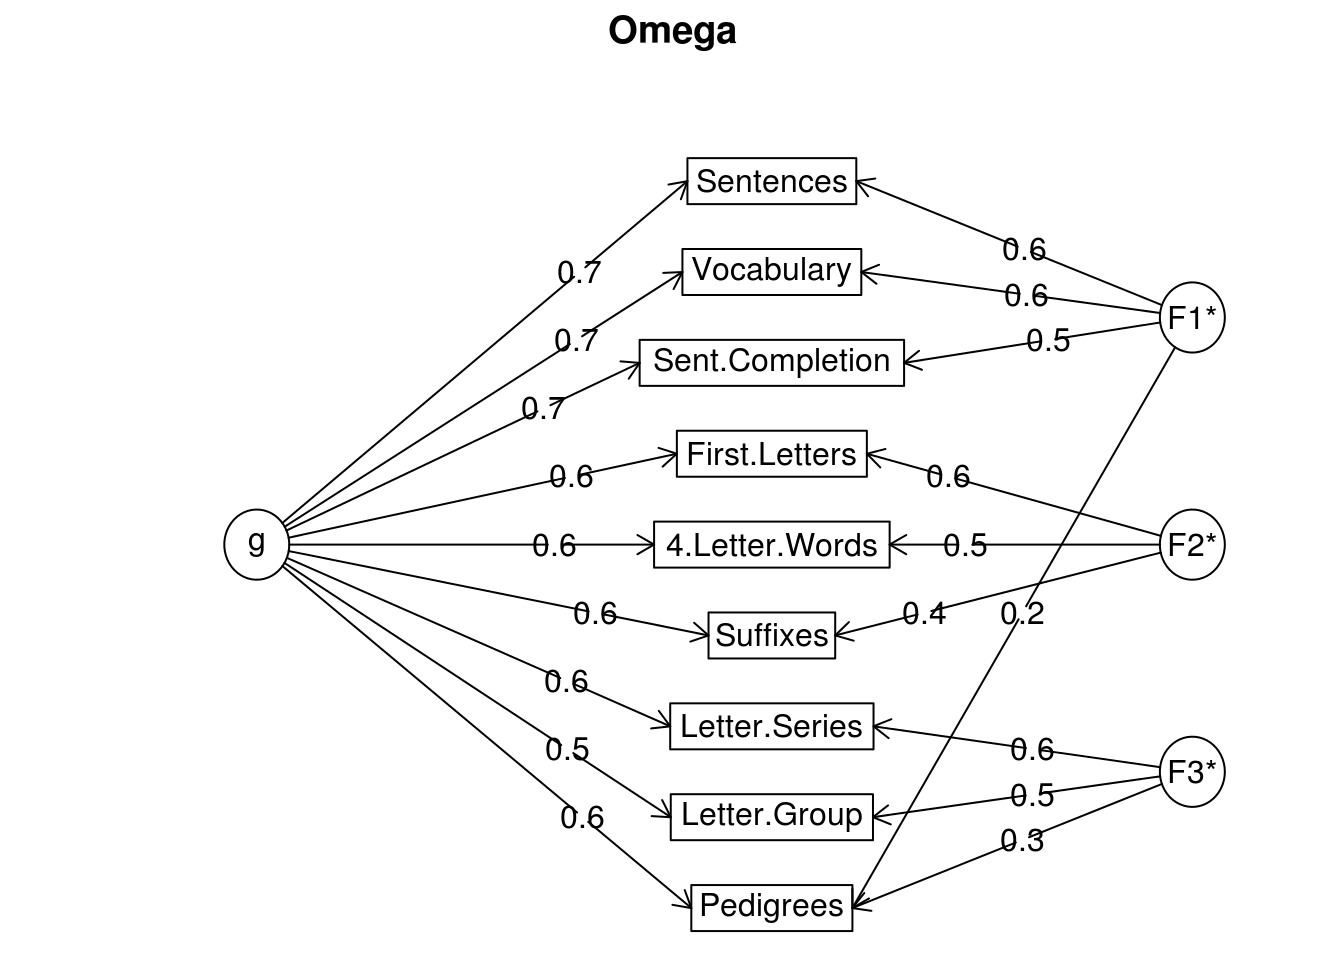
\includegraphics{r-intro-multivar_files/figure-latex/exe_omega-1.pdf}

\begin{Shaded}
\begin{Highlighting}[]
\KeywordTok{round}\NormalTok{(om$omega.group,}\DecValTok{2}\NormalTok{)}
\end{Highlighting}
\end{Shaded}

\begin{verbatim}
##     total general group
## g    0.93    0.74  0.16
## F1*  0.92    0.58  0.35
## F2*  0.83    0.50  0.32
## F3*  0.79    0.47  0.32
\end{verbatim}

\begin{Shaded}
\begin{Highlighting}[]
\CommentTok{#fraction of reliable that is general variance}
\KeywordTok{round}\NormalTok{(om$omega.group[}\DecValTok{2}\NormalTok{]/om$omega.group[}\DecValTok{1}\NormalTok{],}\DecValTok{2}\NormalTok{)  }
\end{Highlighting}
\end{Shaded}

\begin{verbatim}
##     general
## g      0.79
## F1*    0.63
## F2*    0.61
## F3*    0.59
\end{verbatim}

\begin{Shaded}
\begin{Highlighting}[]
\CommentTok{#fraction of reliable that is group variance}
\KeywordTok{round}\NormalTok{(om$omega.group[}\DecValTok{3}\NormalTok{]/om$omega.group[}\DecValTok{1}\NormalTok{],}\DecValTok{2}\NormalTok{)  }
\end{Highlighting}
\end{Shaded}

\begin{verbatim}
##     group
## g    0.17
## F1*  0.37
## F2*  0.39
## F3*  0.41
\end{verbatim}

\bibliography{packages.bib,book.bib}

\end{document}
